%\renewcommand{\tabularxcolumn}[1]{m{#1}}
%\newcolumntype{Y}{>{\centering\arraybackslash}X}
%\newcolumntype{R}{>{\flushright\arraybackslash}X}


\renewcommand{\thesection}{\arabic{chapter}.\arabic{section}}


\chapter{Methodological tools for non parametric functional data evaluation and weather data usage} 
\label{chap:ch1-5}
\cleardoublepage

\doublespacing
\section{Introduction}
In the last chapter, we have introduced a model of supply function equilibria under uncertainty that takes ramping costs into account and we derived solutions that depend on the information the firms have about the future demand at the time of bidding. Here, we will focus on introducing tools that will allow us to perform empirical analysis of the french day ahead market and test these theoretical predictions, which will be the focus of our third chapter.\\

In this short chapter we develop a methodology to analyze data of two specific formats. The focus lies on the methodological details as well as evaluating the performance of our technique. The aim is first to extract points of interests from functional data in order to be able to compare function to one another across bids, and second to describe a methodology that will allow us take into account the uncertainty related to the weather. The economic interpretation is secondary in this chapter. Chapter 3 will use the methodology developed here for a case study of the French electricity market.\\

\section{Point selection on functional data : a non parametric approach}
Reduced form models often rely on exploiting market outcomes for their analysis, i.e. equilibrium prices and quantities, in order to identify the determinants of firm behaviour and test predictions of the theory. On a few markets, sufficient information is available to get around the problem of using endogenous equilibrium data. For example on the government bond markets, both the full aggregate demand and supply functions are observed. This market is of a specific type, it is a divisible goods auction (also called multi-unit or share auctions). These are auctions where multiple units of a good are sold in a single auction. The exact quantity is not predetermined, but endogenous and depends on the price. Furthermore, the auction format is more complex than for indivisible, single unit auctions and most notably requires that bidders simultaneously submit full bid functions for the goods, i.e. multiple price-quantity combinations at which each bidder is willing to buy or sell the goods. The market price and quantity are determined by the intersection of the aggregate demand and supply functions.\\

The aggregate bid functions are very rich in information and the reduced form models can be adapted to use this data. However, the literature on exploiting functional data is limited. This idea has been applied to investigate the determinants of demand bid functions in French government bond auctions \cite{preget2005treasury}. They rely on the propositions first put forward in \cite{boukai1998market} and \cite{berg1999bid}, who identified that aggregate bid functions in divisible goods auctions follow an S-shaped curve that can be estimated by a logistic function. The fluctuations across auctions are claimed to be due to random shocks on the parameters of the estimated logistic function. The methodology is applied in \cite{ozcan2004logistic} to investigate the revenue superiority of the discriminatory price auction format over the uniform price auction format for the Turkish government bonds market.\\

More generally, their methodology consists of a two-stage regression. The first stage summarises the (presumably parametric) functional data of the aggregated demand function as parameters of an estimated smooth logistic function. The second stage reuses the information (concentrated in the estimated parameters) for cross-sectional analyses.\\

Although the auction mechanism is identical to that of the Treasury market and data availability is comparable, logistic function approach does not suit the context of the electricity market due to the strong heterogeneity of the bid functions and their deviations from such logistic shapes, as can be seen in the example of Figure \ref{assymetry}. \\

\begin{figure}[!ht]
\begin{center} \makebox[\textwidth]{
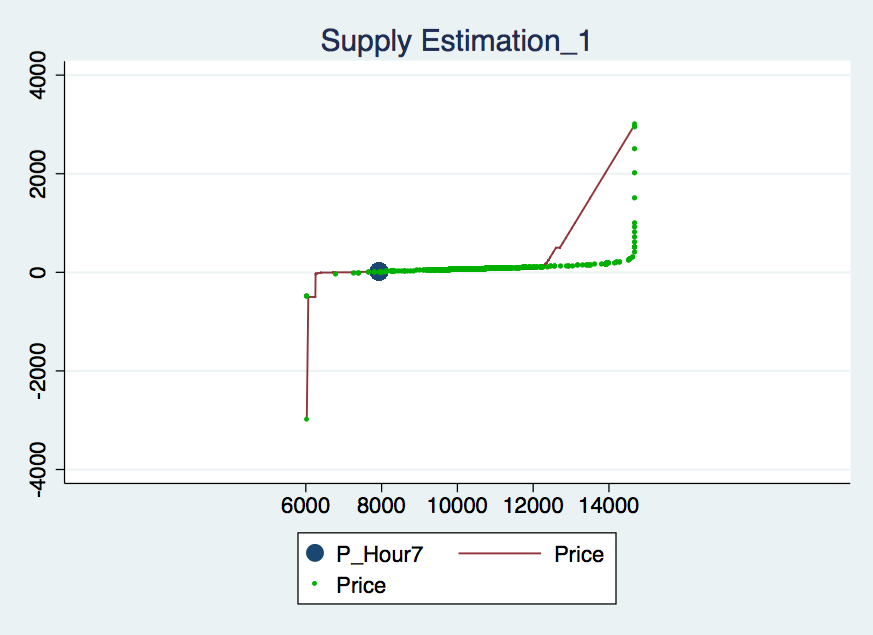
\includegraphics[height=74mm]{figch2/Pic1_C_2011_H7_v30_sym.png} 
} \end{center}
\caption{Example of an assymetric aggregate supply function. The x axis is the quantity in MWh, the y axis if the price in €. In red is the actual aggregate function, in green is an estimated logistic function showcasing the large discrepancies that can arise with this parametric approach. The blue point is the market outcome. }
\label{assymetry}
\end{figure}

The heterogeneity arises from the fact that the bid functions for the electricity auctions are much richer since we have multiple, strategic players on both the demand and the supply side of the market (unlike the market of government bonds, where the supply is monopolistically determined by the Treasury itself). Furthermore, supplier bidding is strongly influenced by the underlying cost of the production technologies. The observed data is consequently less homogeneous and the fitting of the logistic model not convincing. Furthermore, the economic interpretation of the logistic function parameters is very difficult and reducing the whole bid function to two parameters of interest discards a lot of the original information of the bid functions. Finally, we are uncomfortable with the strong assumption of smooth underlying functions and want to circumvent the problems of fitting these.\\

Instead, we develop a non-parametric, functional data analysis approach to select comparable data points from the original bid functions. In our case, this selection of points will yield 4 regions for every curves, each region can be thought of as linear. These selected points are comparable across repetitions of the market (i.e. auctions for different hourly contracts) and can then be used to run a cross-sectional reduced form model. The interest of this approach is threefold. First, it aims to use as much of the original information as possible without distorting it into parameters of a logistic function. Also, information about different parts of the bid function does not influence one another. Second, our approach is “scalable” and as many points as necessary can be extracted. The cross-sectional analyses are then conditioned on the type of comparable points selected. Third, while our analysis provides support for an underlying tri-linear or S-shaped functional form, we do not need to assume a specific functional form nor impose overly simplistic assumptions, such as symmetry of the functional forms, to ensure convergence of the estimator.\\

Here we present the methodology of our point selection and apply it to data from the French electricity market. For now, we ignore specificities of the market for the sake of concentrating on the methodology. We introduce very briefly the data and the market in section \ref{gleinfo}. For a full explanation of the data and the market, we refer the reader to chapter 3. In section \ref{pointselect}, we explain the point selection algorithm. In section \ref{pointresults} we discuss the results of the methodology. Section \ref{pointccl} concludes.

\subsection{Information about our data}\label{gleinfo}

Our methodology is general and can be applied to any market where the structure of data observations is similar. Here, we present and discuss the performance of the method- ology on data from the electricity market. For the purposes of this chapter we will focus only on the statistical properties of the data, not on the economic interpretation.\\

We apply our methodology to data from a divisible goods auction. In this auction, each buyer and seller submits a full individual bid function, i.e. a demand or a supply function, which consists of 2 to 256 monotone price-quantity combinations. The final bid function consists of these explicitly submitted bid points and all linearly interpolated points between them.\\

The market is cleared by computing the intersection of the aggregate demand and aggregate supply functions, which are each obtained by summing up all individual bid functions for the demand and supply side of the market respectively. In a uniform pricing format, the determined equilibrium price is applied to all units sold in that auction.


\subsection{Point selection algorithm}\label{pointselect}

To briefly fix ideas, let's assume that we are interested in a regression \`{a} la: 
$$ S' = \alpha + \boldsymbol{\beta  X} + \epsilon$$
where $S'$ is the steepness of the bid function, $\boldsymbol{X}$ the stacked vector of exogenous variables (not specified further here), $\alpha$ the regression constant, $\boldsymbol{\beta}$ the stacked vector of regression coefficients and $\epsilon$ the error term. \\

The information $S'$ is drawn from the bid functions of a %the electricity 
market, and varies along the different points of the bids.\\

For comparability, we require that a chosen point $k$ from a supply function must be comparable to the $k^\text{th}$ point from the supply functions of another auction. The same goes for chosen points of the demand functions. The reason for this assumption is that comparing those points accross auction allows us to describe how the functions, that is the aggregate strategies, change shape when our independant variables vary. Note that we do not impose comparability between a pair $k$ of points from a supply and a demand function of the same auction. 

 
\subsubsection{Non-parametric technique to compare bid functions}
\label{comparablepoints}
Consider two demand functions (as shown in figure \ref{comparedfunc}). 
\begin{figure}[!ht]
\centering
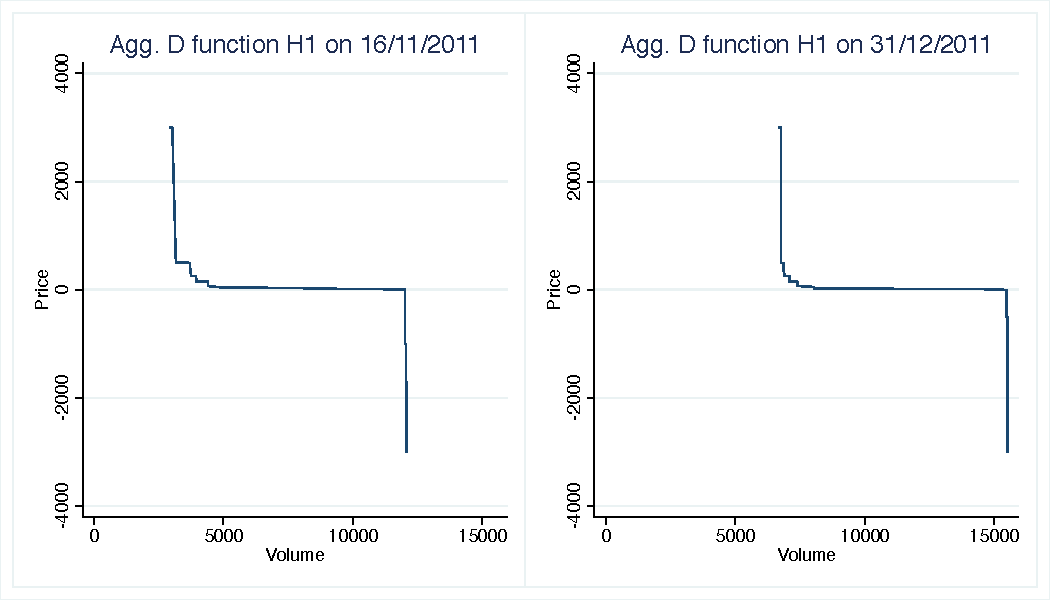
\includegraphics[trim=0.1cm 0.1cm 0.1cm 0.1cm, clip=true, height= 60mm]{figch2/compare2d.pdf}
\caption{Comparison of two aggregate demand functions for the same hour}
\label{comparedfunc}
\end{figure}
 We have to identify "features" of the different functions in order to determine which points can be compared to one another. We aim to reproduce the type of analysis that the brain performs automatically when faced with such curve: we clearly identify three regions of different slope, where the central region is less steep than the left and right regions. \\

To recognise these features, we perform two successive kernel density analyses\footnote{Bandwidth in the first estimation $=45$, bandwidth in the second estimation $=2$, kernels: epanechnikov.}. 
For details on the bandwidth and kernel selection as well as algorithm specificities, see appendix \ref{implementingkernel}. This allows us to access estimates of the absolute values of the first and second derivatives of the demand functions as shown in graphs B and C of figure \ref{selectedpoints}.\\ 
\begin{figure}[!ht]
\begin{center}
\makebox[\textwidth][c]{
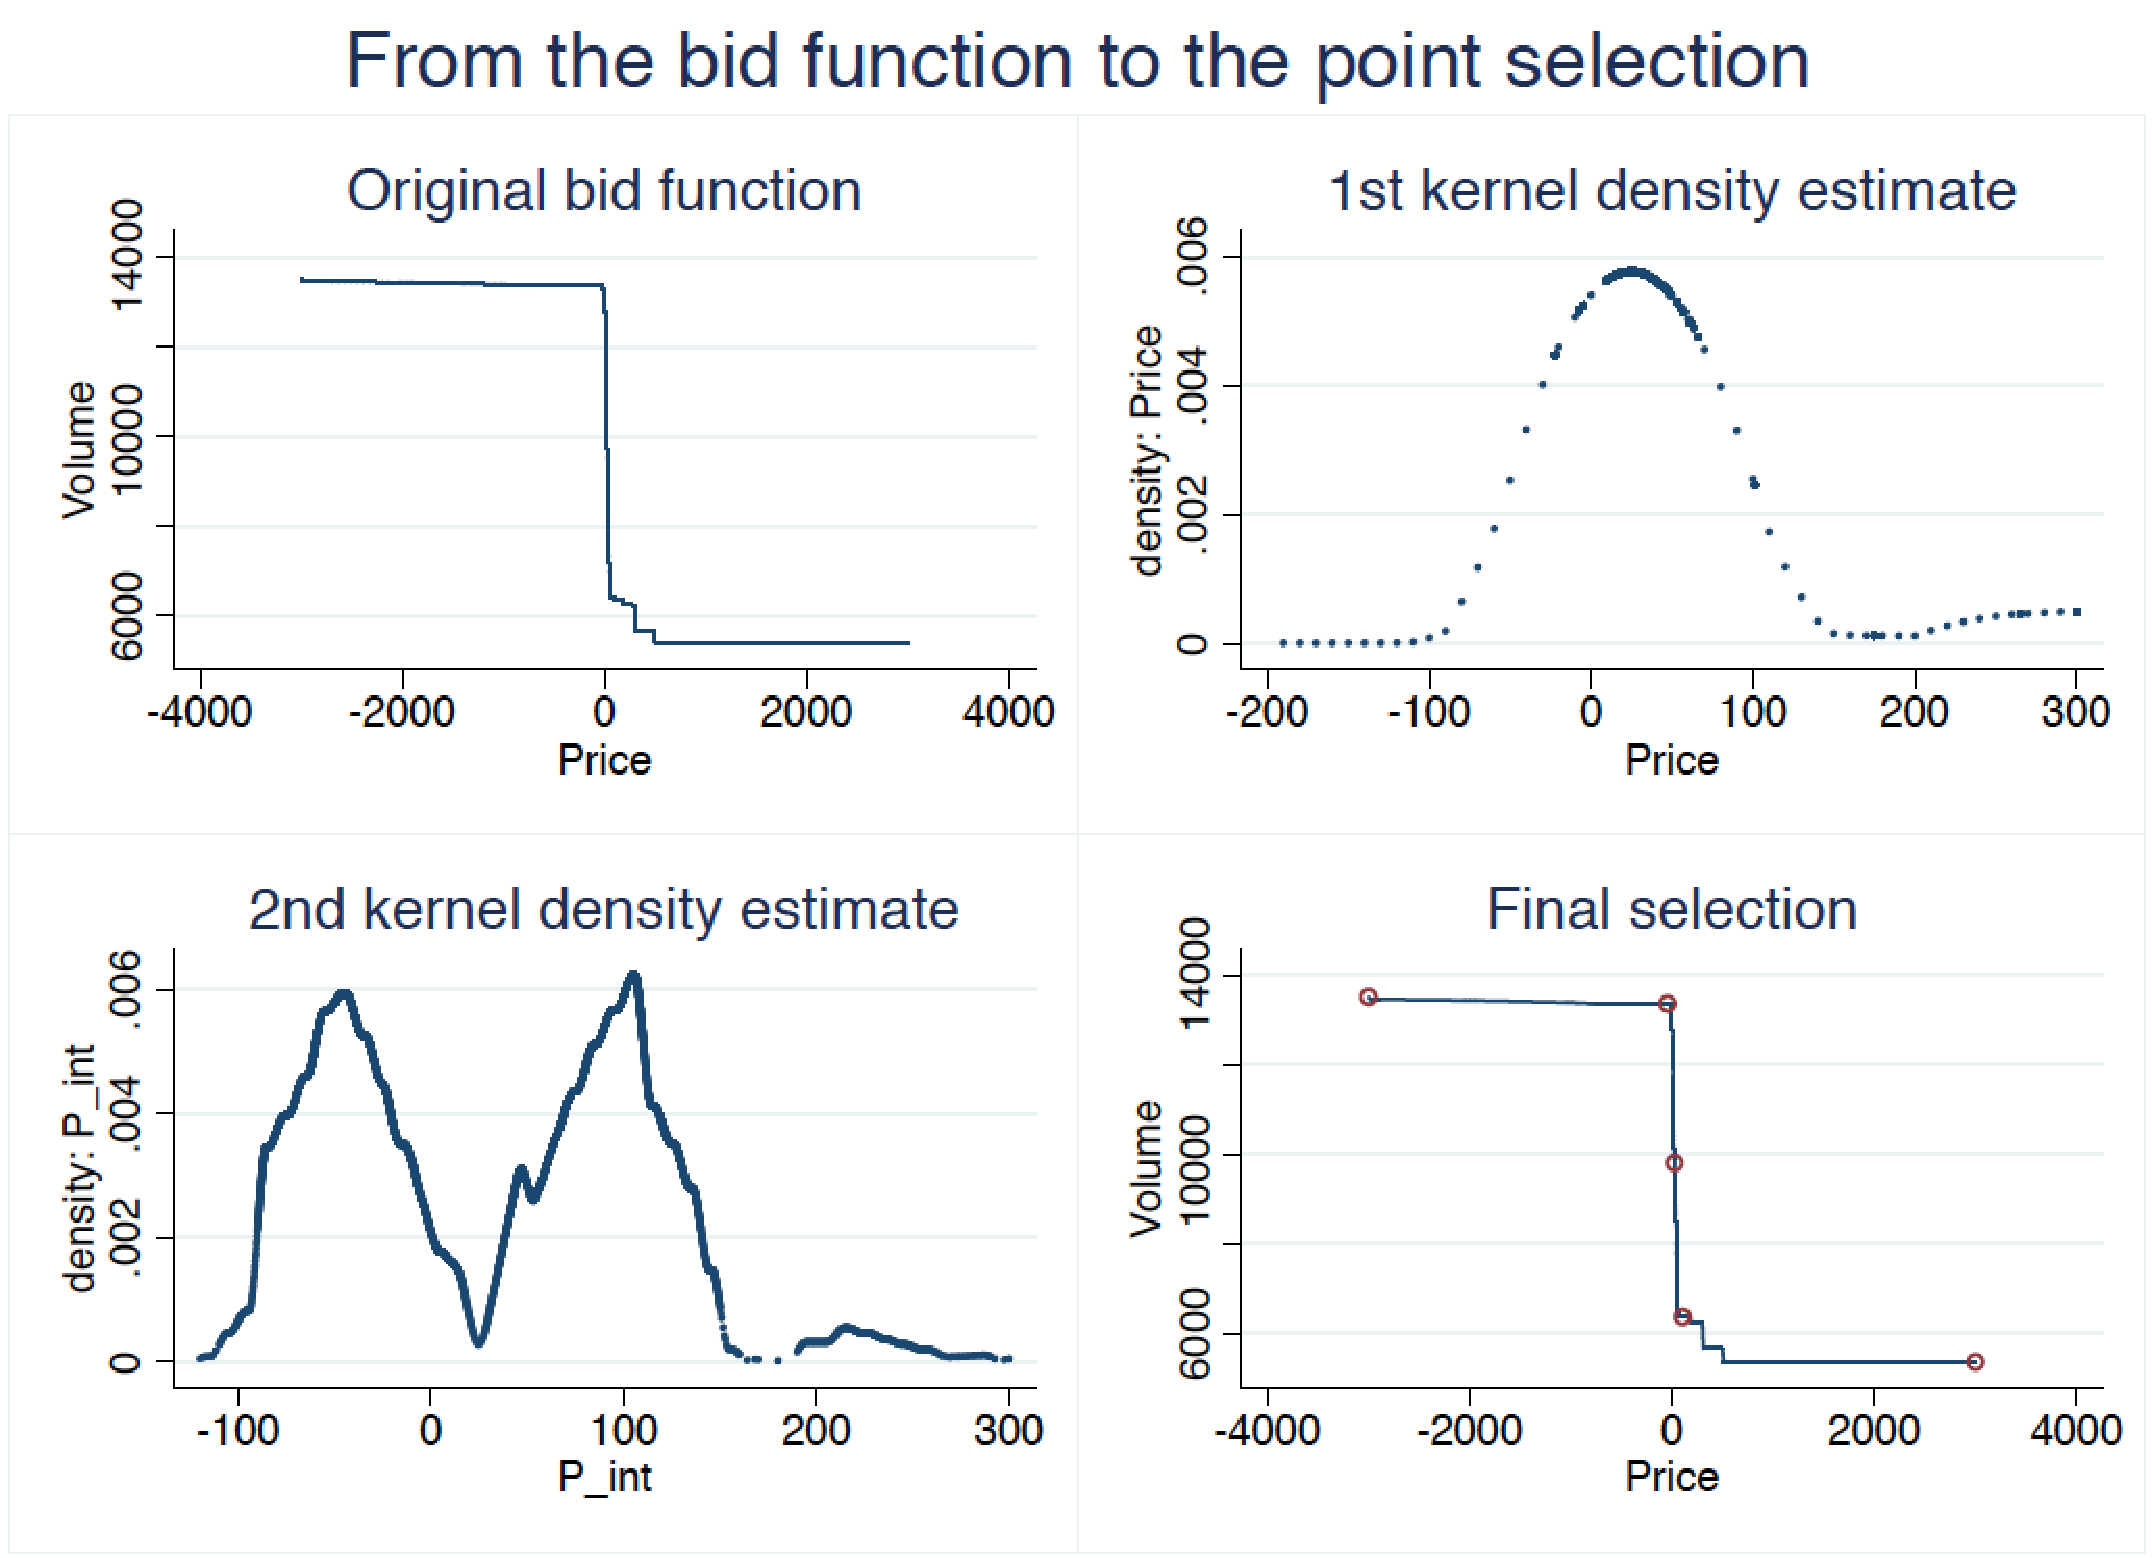
\includegraphics[height= 95mm]{figch2/Shot30.pdf}
}
\caption{Steps of the point selection process}
\label{selectedpoints}
\end{center}
{\small Top left (A): The full original aggregate demand bid function for hour 8 on 15.01.2011 in the quantity - price dimension. Top right (B): Kernel density estimates of the first derivative, zoomed on the relevant price range. Bottom left (C): Zoomed kernel density estimates of the second derivative. Bottom right (D): The full original bid function with the $K=5$ selected points. 
}
\end{figure}

We are therefore able to identify the regions of very high curvature, which define the transition between the three characteristic regions of these functions. We assume that these maxima can be compared across different auctions. This hypothesis is commonly made in functional data analysis and known under the method of landmark registration \cite{ramsaysilverman2005functional}. This has been applied in \cite{wolfi2013interacting}, chapter 4, to day-ahead electricity data, in order to identify the effect on fuel price shocks on supply curves. However, this landmark registration was applied in a parametric form : the regions of high steepness were identified as any part of the curve above 90€/MWh. \\

We can develop this method further and define intermediary points\footnote{As an example, we could extract those points corresponding to half the density value of the maximum density of the second order derivative. The four points selected (one for each monotone portion of the graph of second derivative estimates) would then correspond to those where the curvature of the function is halved. Together with the maximum, the additional point would contain information on the speed (radius of the curvature) at which the function changes.} that can again be compared to one another. This method allows to define as many points as needed, for computational reasons we limit ourselves to $K=5$ points\footnote{The point selection algorithm took 2 weeks runtime to complete its task of selecting 5 points per function. Defining intermediary points would have taken disproportionately more time since many sorting and interpolation steps are necessary for each intermediate point.}. \\

Graph D of figure \ref{selectedpoints} visualises an original demand bid function and the selected points that we retain as an informative summary of the original curve. Once this work is done we are left with $K=5$ points per observed aggregate function, those points defined in such a way that they can be compared from one auction to another. \\

In our setting, the selected points are the two end-points of the curves (where bidding is imposed by the auction rules at the minimum $(k=1)$ and maximum $(k=5)$ Price), the point corresponding to what can be thought of as the point of inflection (determined by the maximum of the first derivative, $(k=3)$ in the plane $(p,q)$) and the points separating the regions of high and low elasticity in price (determined by the maximum second derivatives to the left $(k=2)$ and right $(k=4)$ of the POI). \\

We described the technique here for the case of a demand function. The information measured at these points can thereby be compared across demand bid functions of different auctions. The method is used analogously for selecting comparable points on the supply function. We are hence able to extract slopes at these selected supply bid points, which are again comparable across auctions.\\


\subsection{Results of the point selection methodology}
\label{pointresults}

\subsubsection{Precision of point selection}
We have selected $K=5$ types of comparable points for each of the $37500$ demand and supply functions present in our dataset. This section details the results of the point selection methodology and presents evidence why the point selection algorithm has produced comparable points reliably. \\

The graphs in figure \ref{g10el} %and \ref{g10hl}
 show the local density of selected points in the price - quantity space for the demand (left) and supply (right) curves.
The fact that the groups of data points are disjoint from one another indicates that the points selected are distinctly different across groups. \\

\begin{figure}[!ht]
\begin{center}
\makebox[\textwidth][c]{
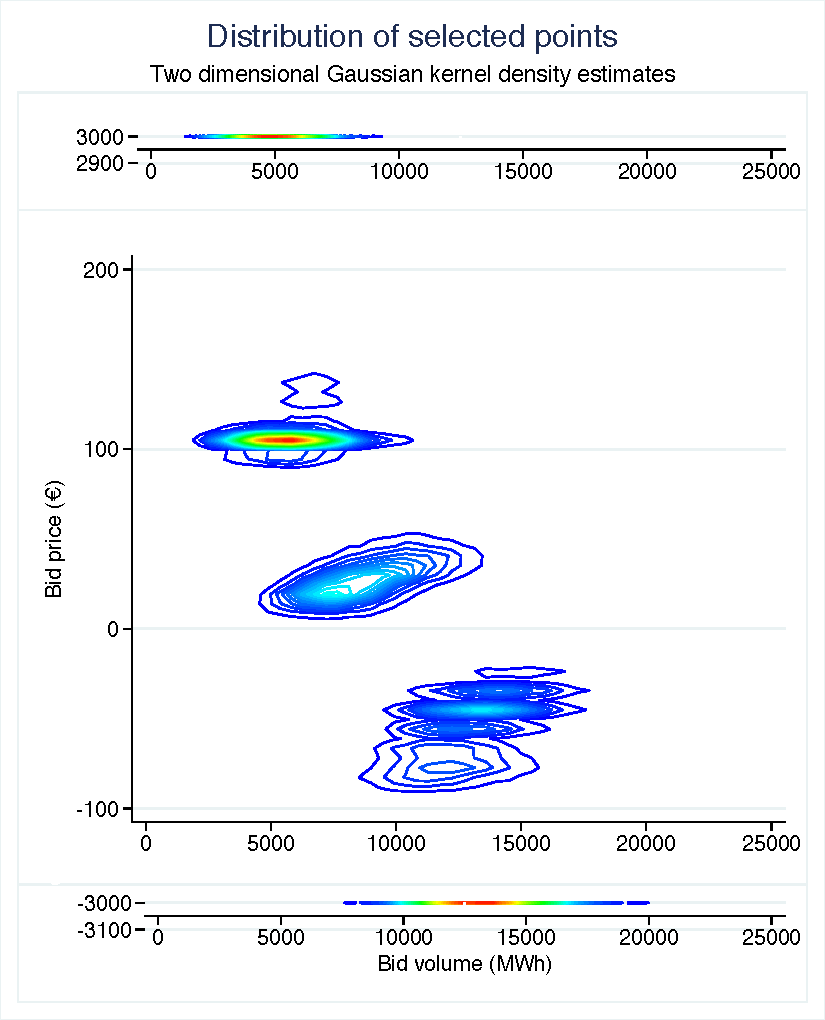
\includegraphics[trim=0cm 0cm 0.4cm 0cm, angle=0, clip=true, height=100mm]{figch2/g10el.pdf}
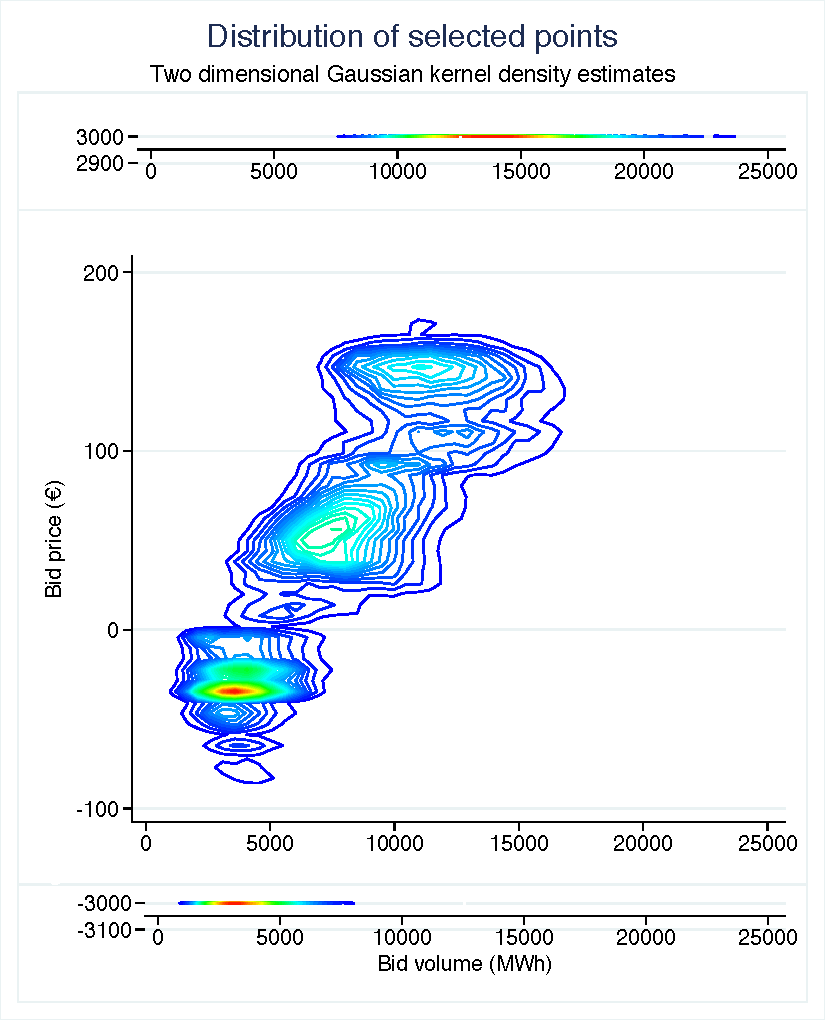
\includegraphics[trim=0.35cm 0cm 0cm 0cm, clip=true, height=100mm]{figch2/g10hl.pdf} 
} 
\caption{Heat map on selected, comparable demand and supply points}
\label{g10el}
\end{center}
{ \small Note: Please note the discontinuity in the scale of the y-axis. The three seperate graphs are arranged to be understood as a single one. The warmer the colours of the heat map, the higher the frequency of selected price-quantity pairs. The colour legend is omitted for brevity, density changes between contours are of the order of $10^{-4}$.} 
\end{figure}


In figure \ref{g10el}, selected points of type $k=1$ manifest at the bottom of the graph with prices fixed at $-3000$\euro /MWh. Similarly, $k=5$ points appear at the top of the graph with prices fixed at $+3000$\euro /MWh. The three distinct groups of data points refer to points of type $k=4$, $k=3$ and $k=2$, respectively, when reading the zoomed, center part of the graph from top to bottom.\\

We note that the point selection for the demand curves has produced groups of points that are more distinct (and thus more robustly attributed to a certain type $k$) then for the supply function. \\

Our methodology only relies on assuming that the first derivative is uni-modal and that sufficient variation exists in the data to distinctly identify the regions of different slope. Overall, this is strong evidence that the algorithm is able to distinctly differentiate between points of different types. \\

\subsection{Observations of bidding frictions}
Distinct point selection is further supported by the evidence in figure \ref{patternsgraph}. These graphs show the distribution in the price-quantity space of the selected points separately for the demand and supply function. Distinct clouds are an indication that selected points are different across types $k$.\\

\begin{figure}[!ht]
%\begin{center}
\makebox[\textwidth][c]{
%\includegraphics[height=65mm]{g10b2.pdf} 
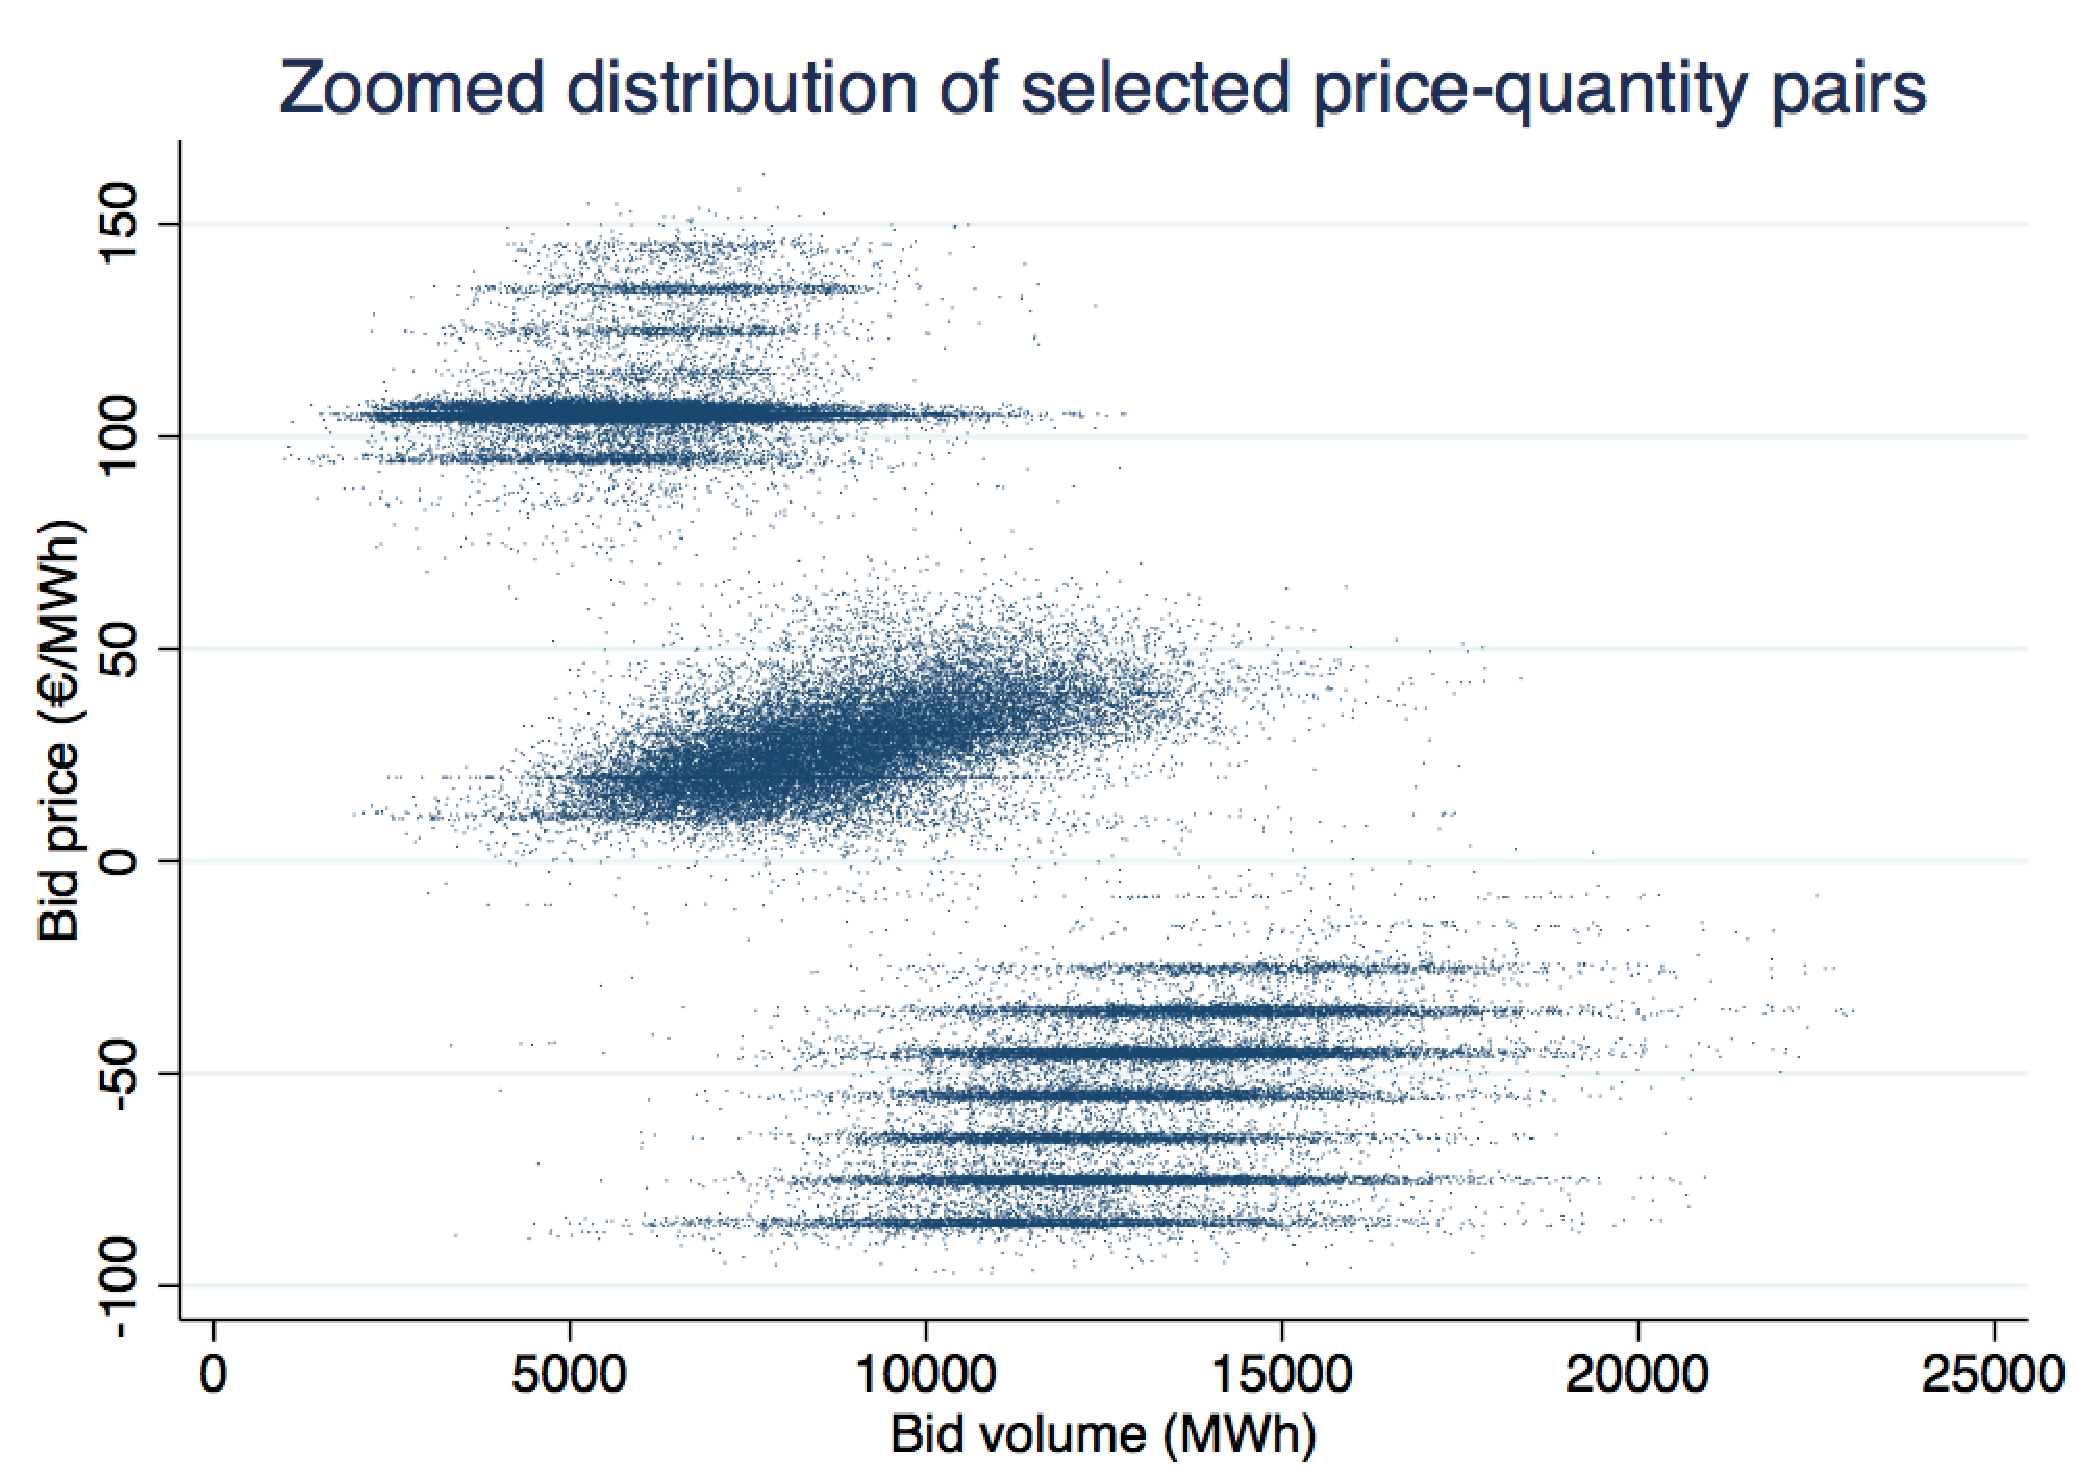
\includegraphics[trim=0cm 0cm 0cm 2.5cm, clip=true, height=48mm]{figch2/Shot06.pdf} 
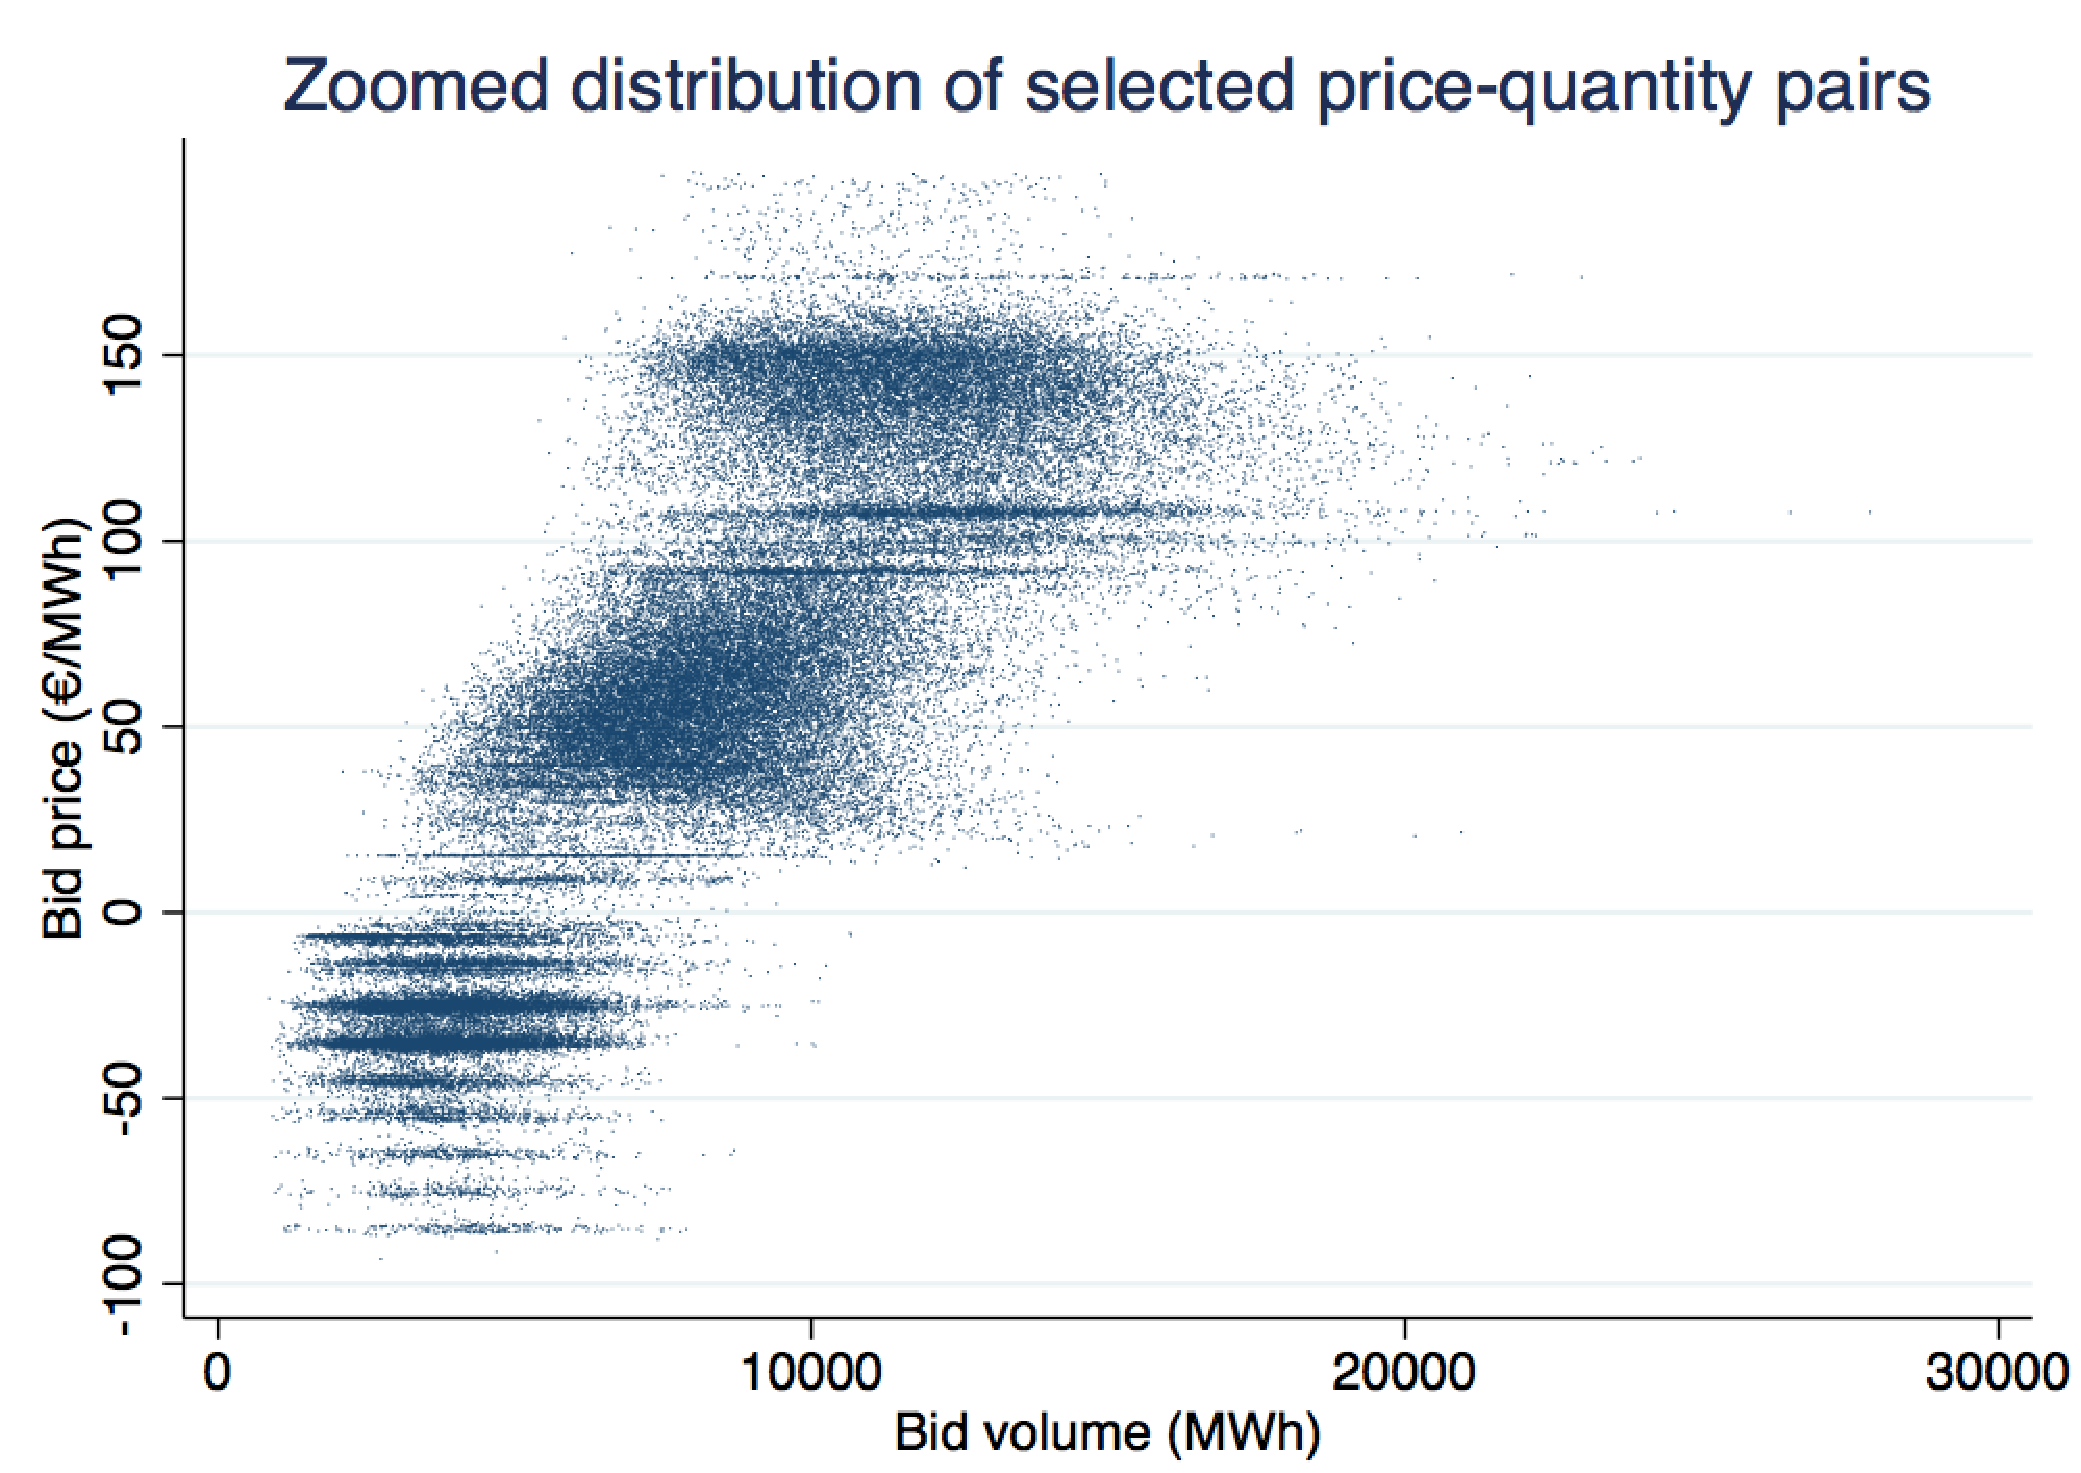
\includegraphics[trim=0cm 0cm 0cm 2.5cm, clip=true, height=48mm]{figch2/Shot15.pdf} 
}
\caption{Distribution of selected demand (left) and supply (right) points}
\label{patternsgraph}
%\end{center}
%{ \small Note: This graphs shows the zoomed distribution of the selected points in comparison to the heat map in figure \ref{g10el}.} 
\end{figure}


However, a feature of the graphs is striking: patterns (horizontal lines) seem to exist for the selected points of type\footnote{Types $k=1$ and $k=5$ do not exhibit variation in price, because bidding at the extreme prices of  +-3000\euro{}/MWh is imposed by the auction rules. We thus neglect their analysis here.} $k=2$ and $k=4$. Many selected points accumulate at certain prices of regular intervals of 10\euro{}/MWh, i.e. there seem to be focal price points for the bidders at the curvature points of the bid functions. The pattern is present for selected points of both the supply and demand functions, although the selected points from the supply function exhibit this pattern slightly less. \\

The points following the pattern (types $k=2,4$) represent the points of maximum curvature of the aggregate bid functions, i.e. the region where the aggregate bid function transitions from a price elastic center portion to the price inelastic extremities of the bid function. \\

%While we do no have a story for this phenomenon, 
Without prioritizing any explanation\footnote{ We do not investigate the origins of bidding frictions in this section, we focus purely on  the methodology. For the electricity market, a few possible explanations are that (1) bid functions are driven by marginal costs consideration towards the extremes of the bid curve, (2) bidders bid coarsely since the have used up much of their bid point allowance (256 points) on the center portion of the curve, (3) bidders spend less effort on adequately bidding at extremes since the likelihood of the market outcome occurring at the extremes is much lower. }, we acknowledge the existence of bid point patterns in the values (i.e. prices and quantities) of selected points. \\

We are, however, interested in $S'$, the slope at each selected point - an information measured at the selected point. We therefore investigate whether the values of the first derivative at the selected points display a pattern. Figure \ref{histpattern1} shows the histograms of slopes of supply functions for the points $k=2,3$ and 4. No pattern in the values of the derivatives is apparent. \\

\begin{figure}[!ht]
\begin{center}
\makebox[\textwidth][c]{
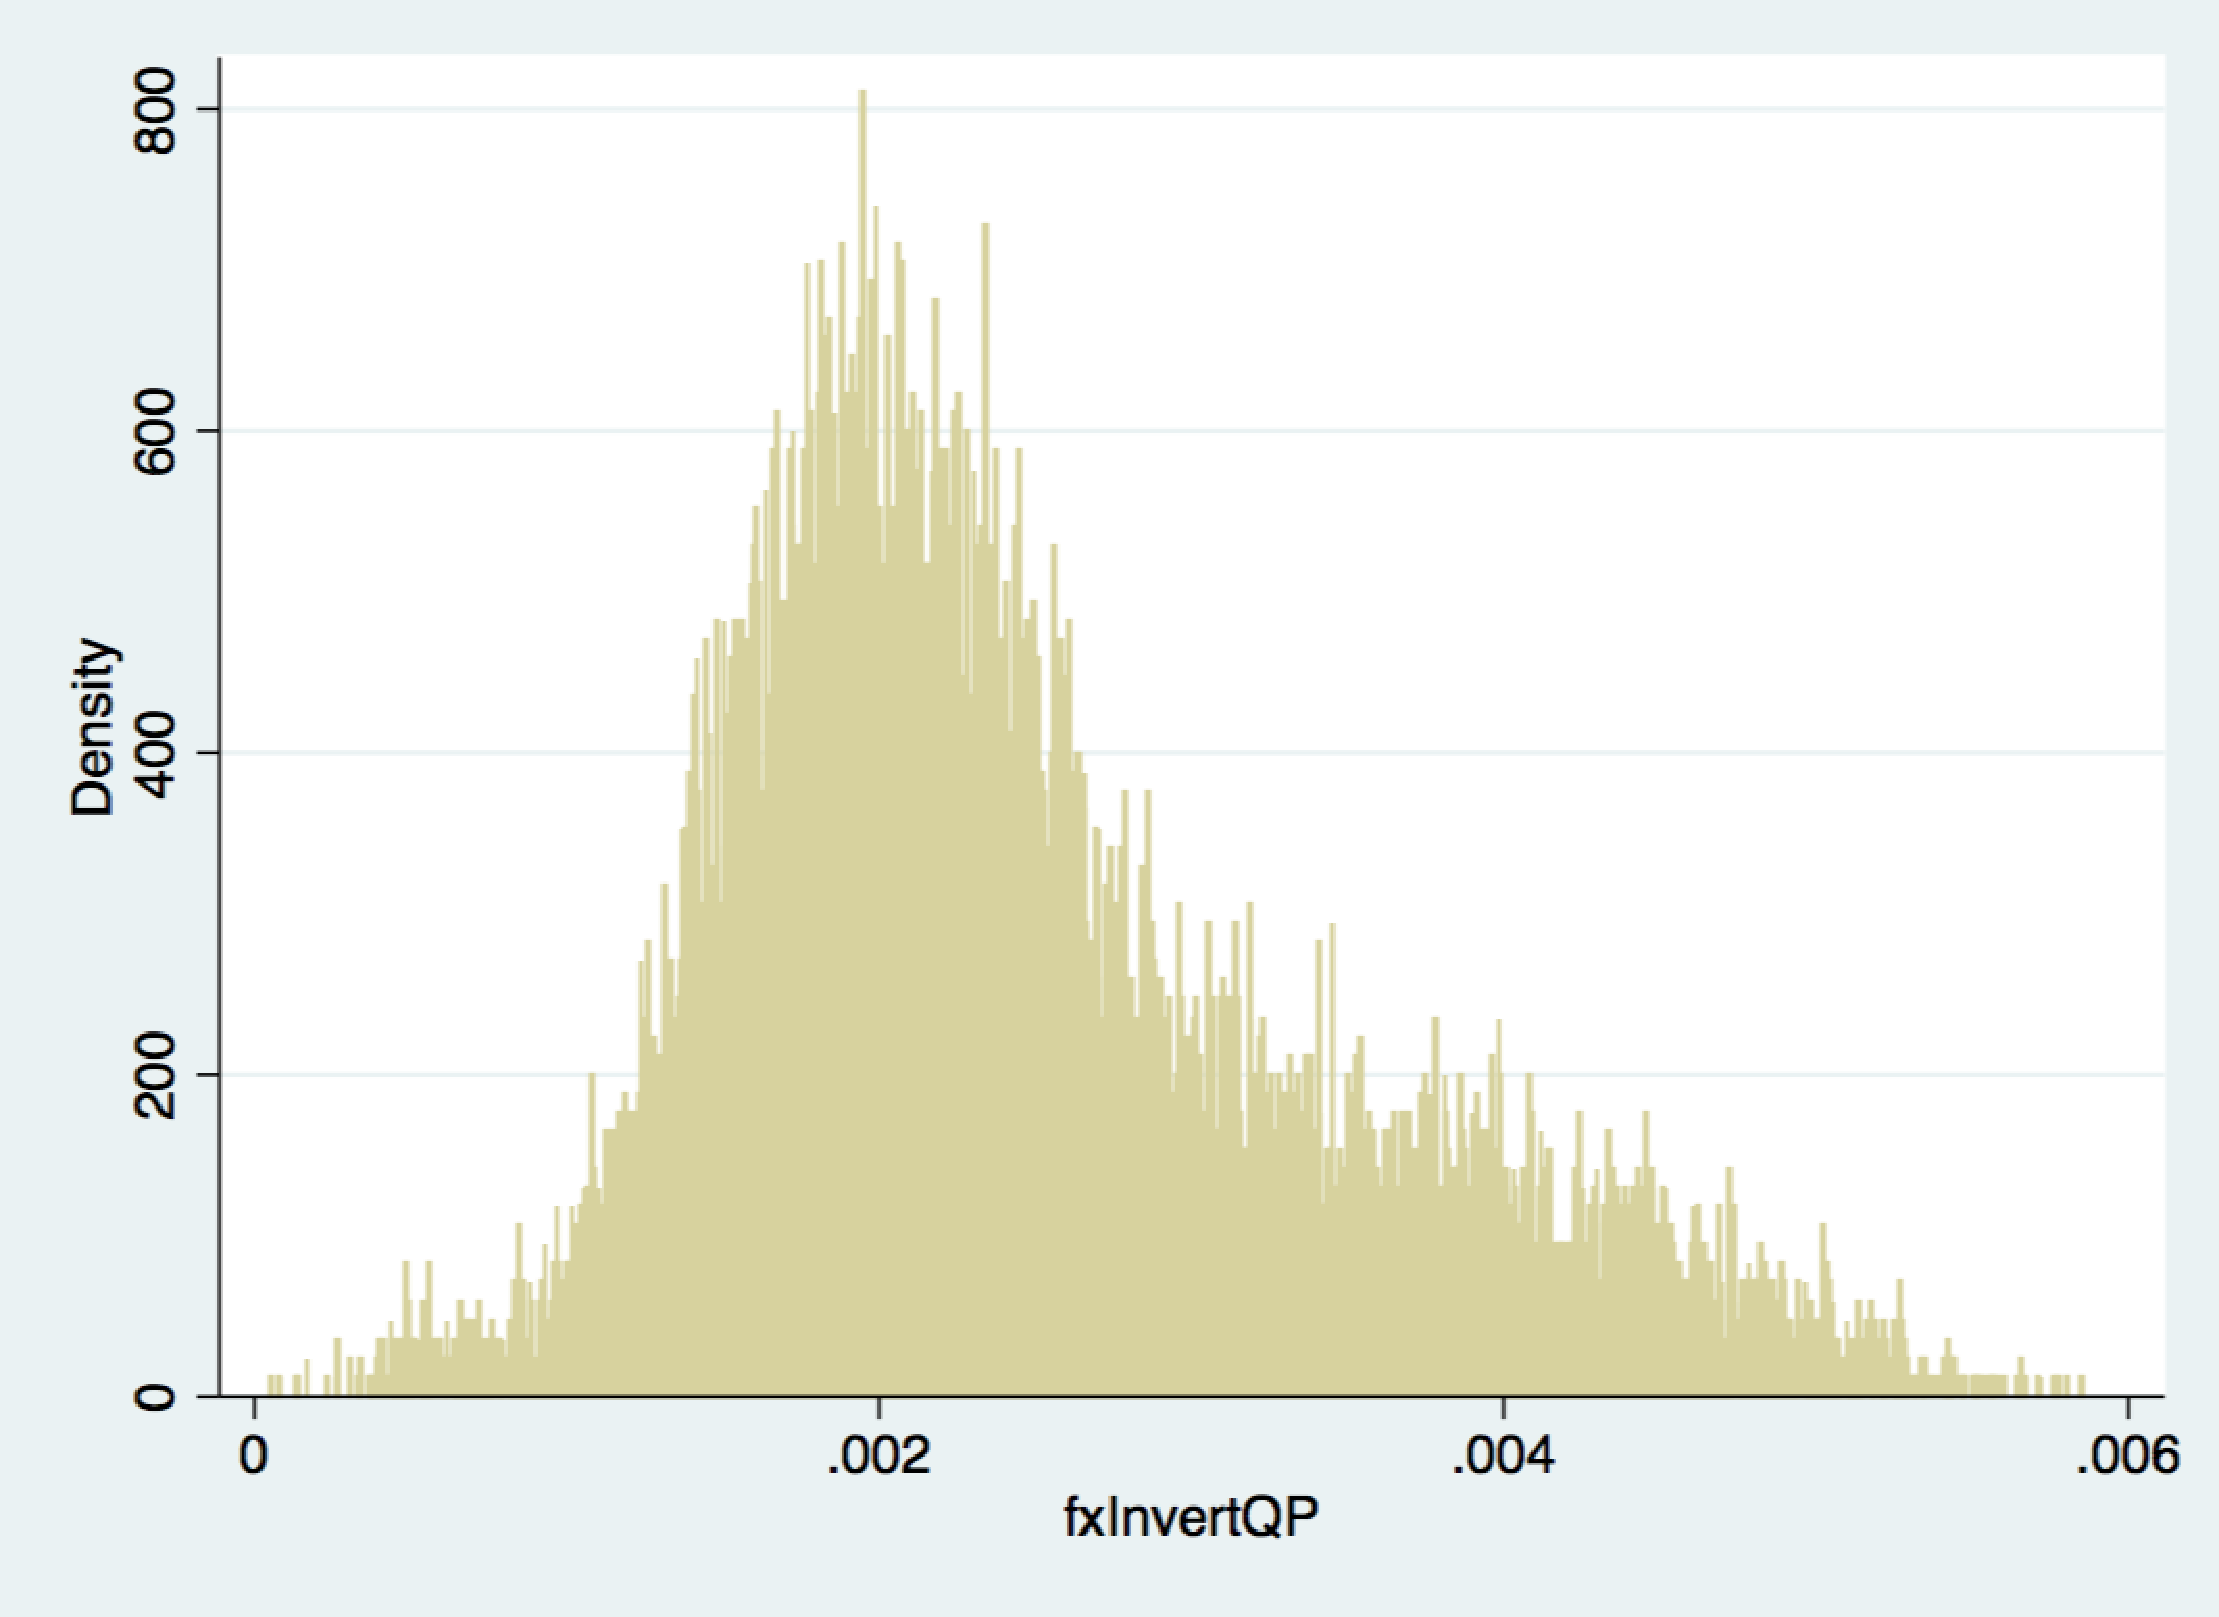
\includegraphics[trim=0cm 0cm 0cm 0cm, clip=true, height=35mm]{figch2/histslope3.pdf} 
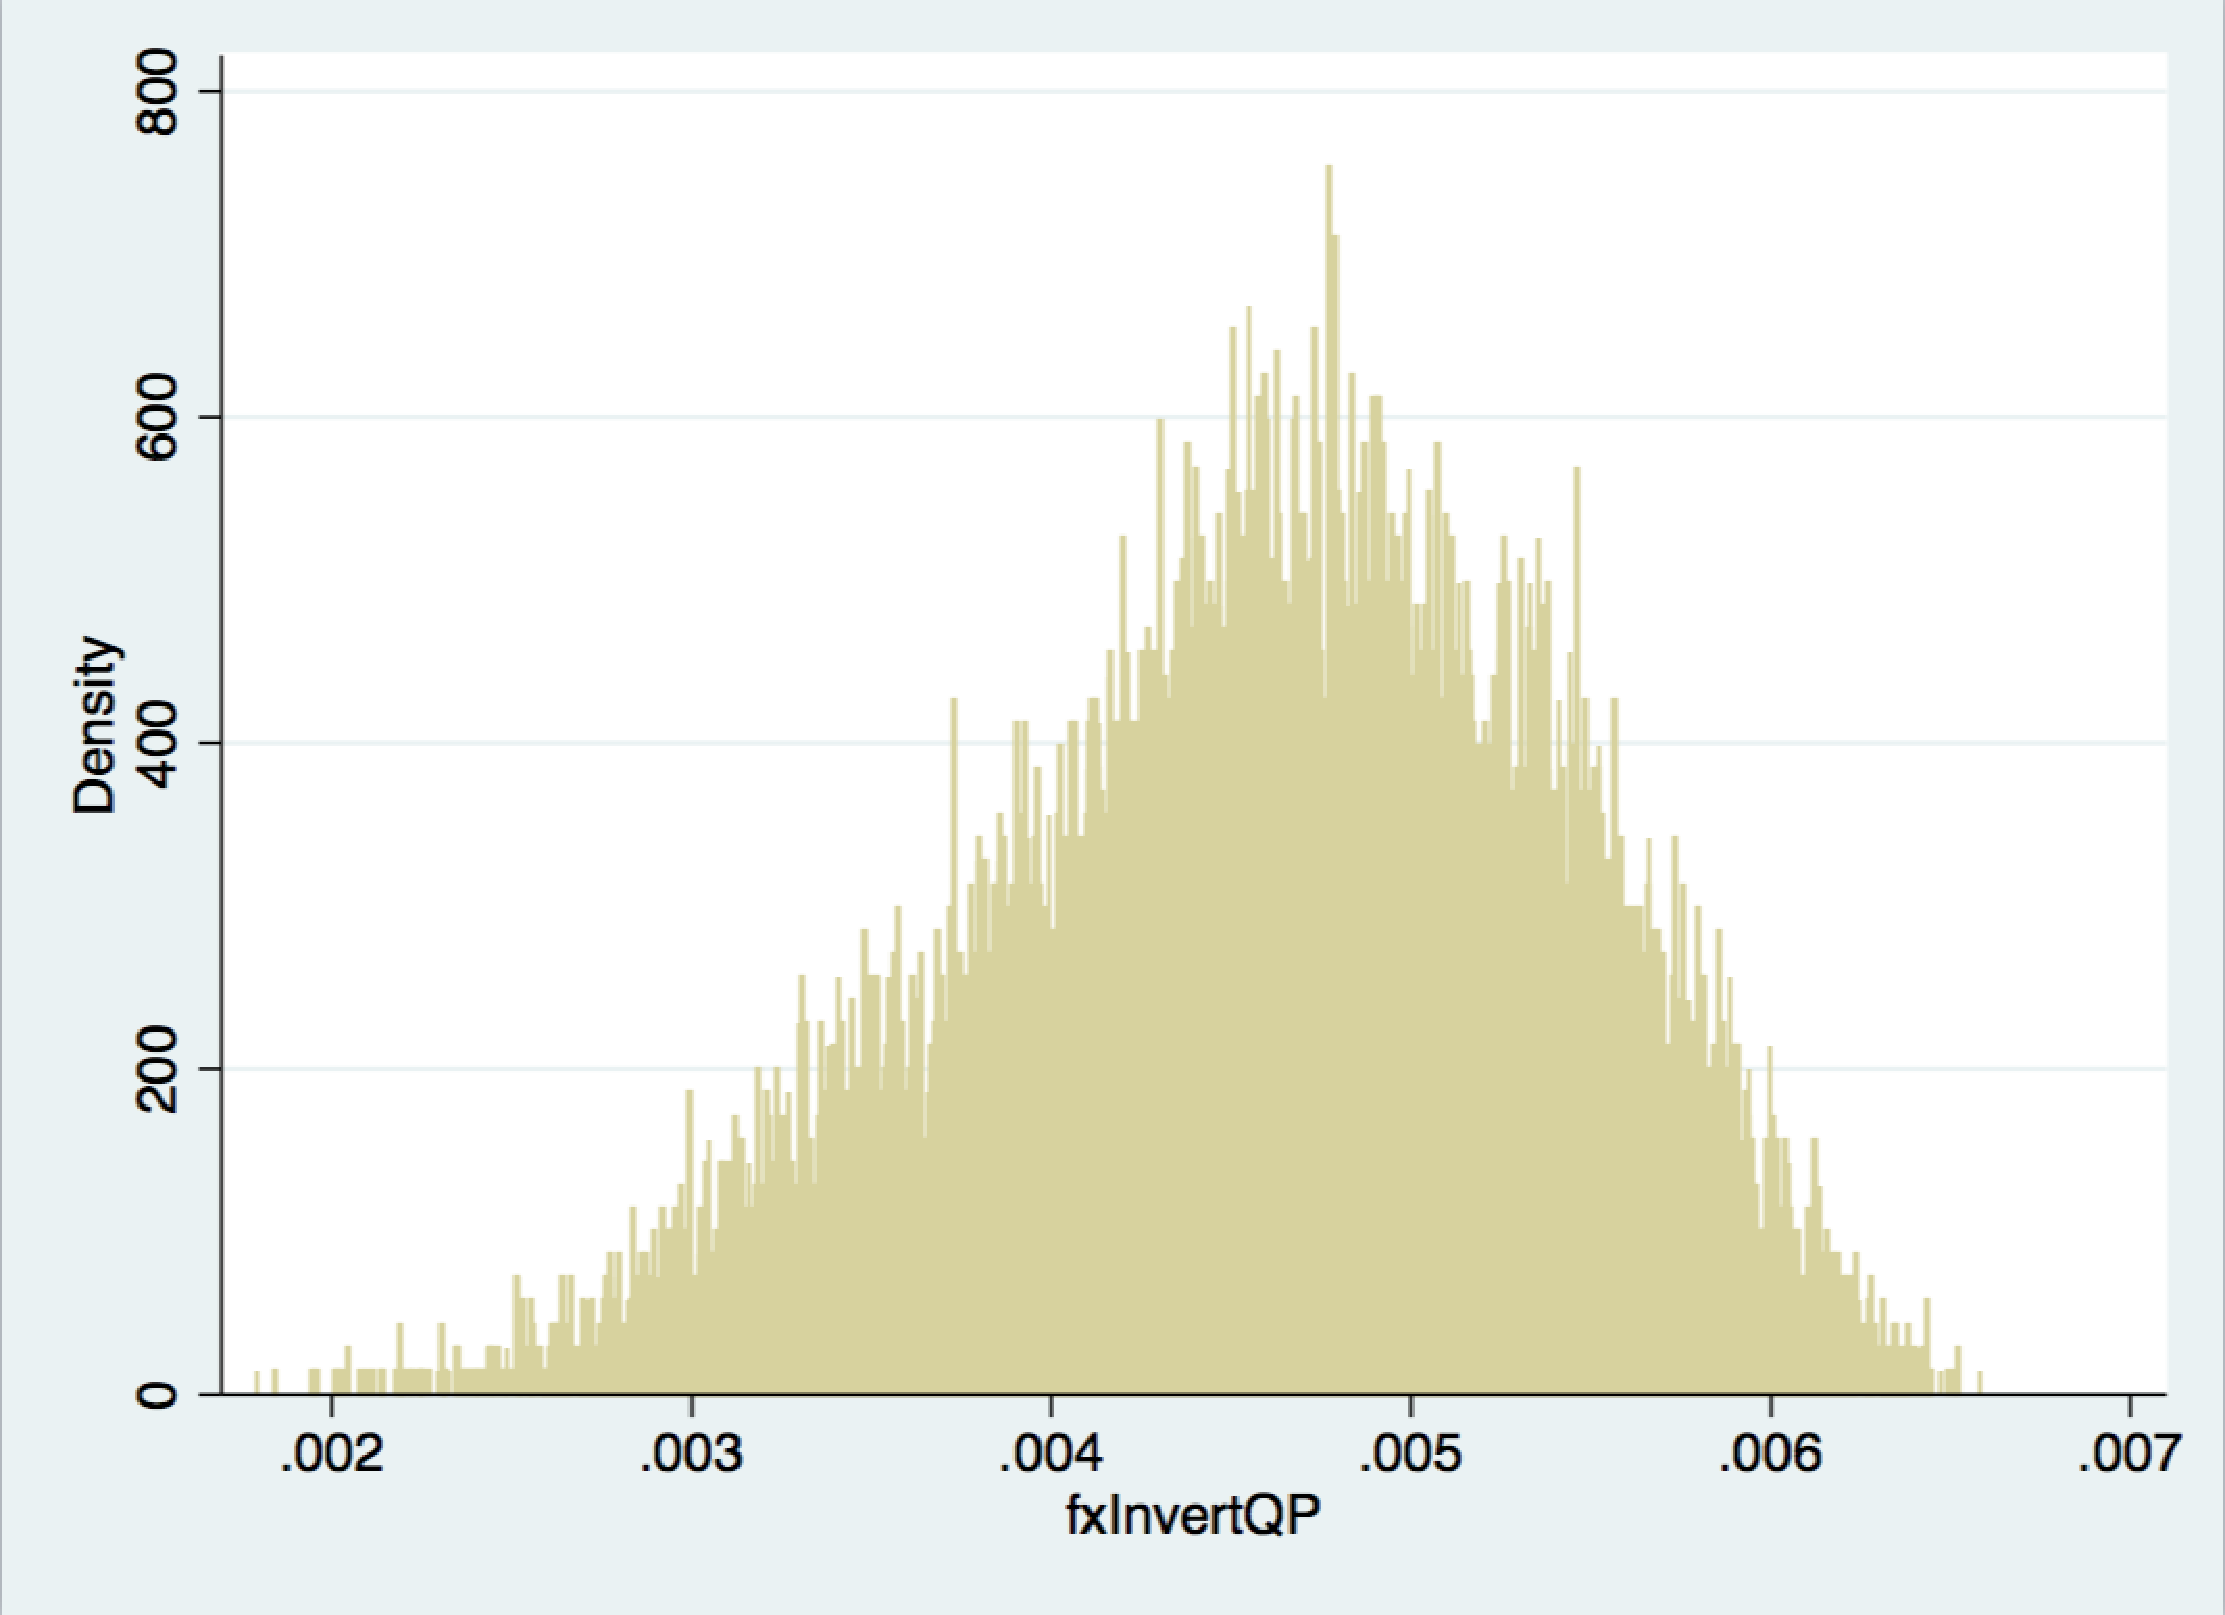
\includegraphics[trim=0cm 0cm 0cm 0cm, clip=true, height=35mm]{figch2/histslope5.pdf} 
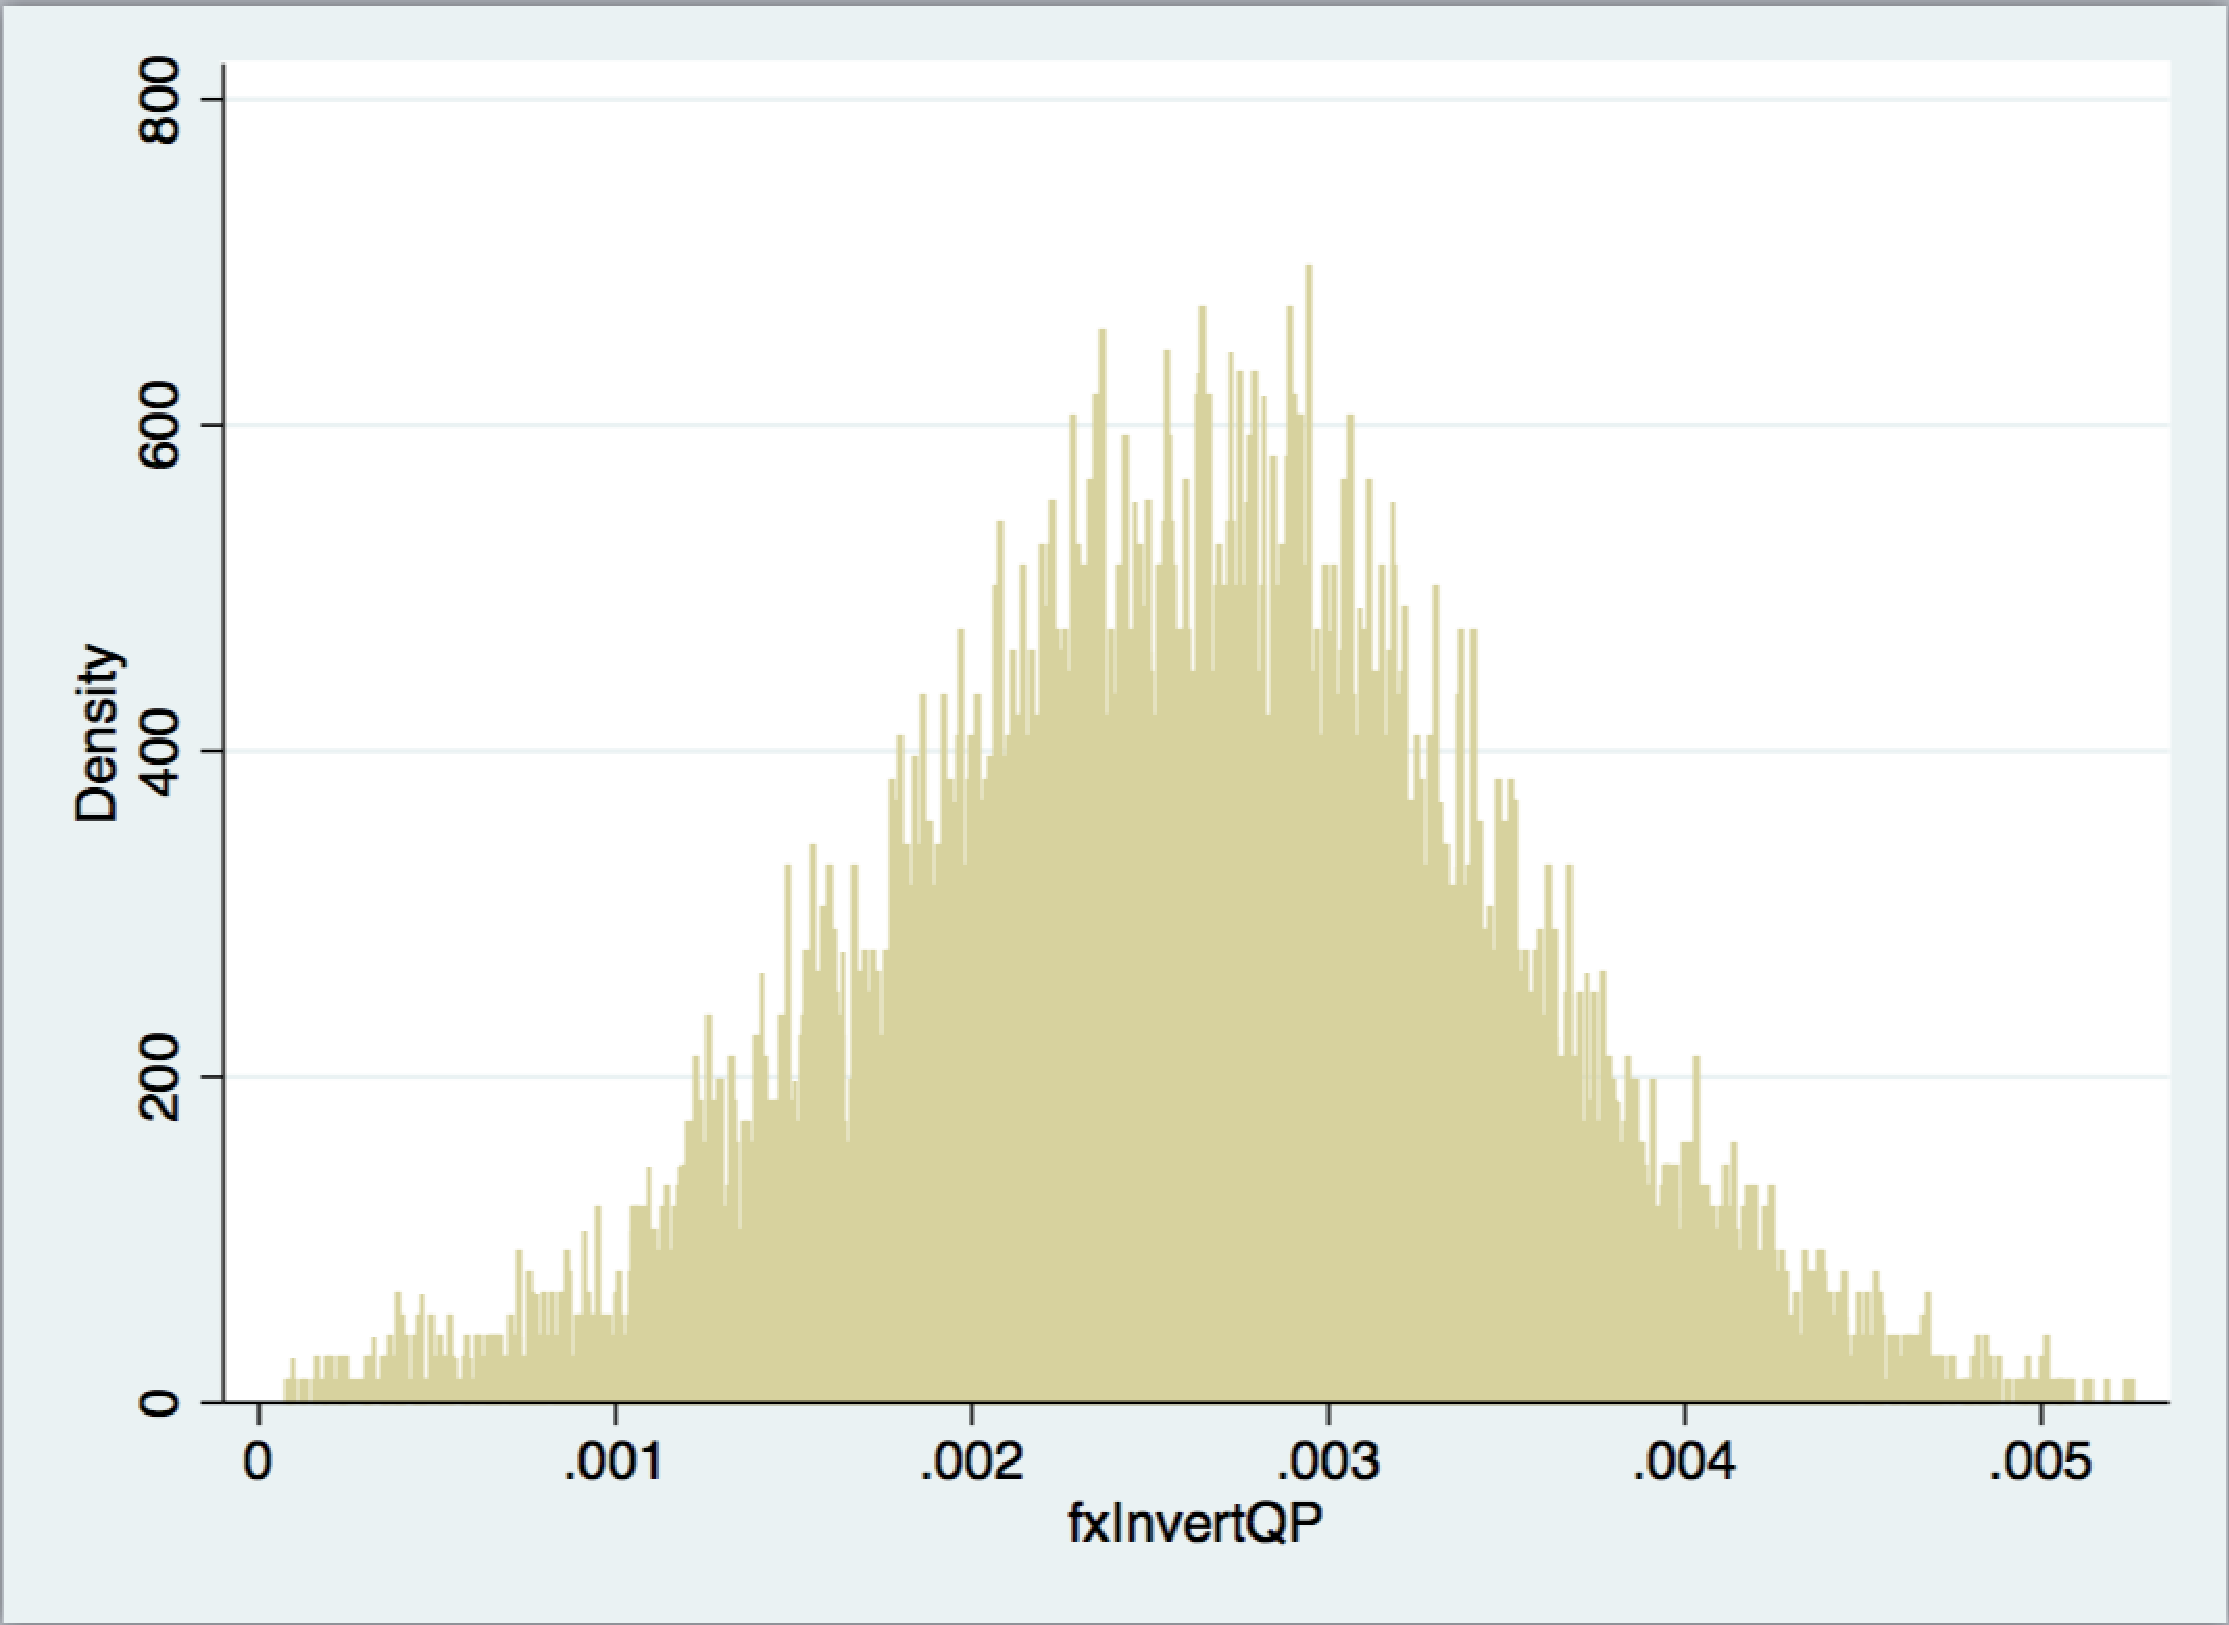
\includegraphics[trim=0cm 0cm 0cm 0.1cm, clip=true, height=35mm]{figch2/histslope7.pdf} 
}
\caption{Histogram of slopes per point type}
\label{histpattern1}
\end{center}
{ \small Note: Histograms of extracted slopes at points of type $k=2$ (left), $k=3$ (middle) and $k=4$ (right).} 
\end{figure}
% STATA COMMAND: hist fxInvertQP if select==7, bin(1000)


Although values of the selected points are possibly biased due to focal price points, we do not observe patterns in the variable of interest (i.e. the first derivatives of the selected points) and deem the methodology adequate for our purposes. \\

Finally, we emphasize that the observed patterns are not caused by the point selection mechanism since the algorithm can only choose between explicitly bid points or linearly interpolated points, that could be part of a market equilibrium under the reigning price setting algorithm. The pattern arises from many horizontal steps occurring at the same prices in different auctions. 


\subsubsection{Value of selected points (determining $K$)
%Degrees of freedom of the inferred bid function
}
We remind the reader that the aim is to recover points that summarize well the behaviour of the full aggregate bid functions in different auctions. 
Our technique allows us to extract representative and comparable points across bid functions of different auctions. Form the selected points, we can also go back to infer the original bid function from which the points were selected. In order to evaluate the utility of our methodology, we investigate the added benefit of an additional point in our point selection. \\

By selecting $K=5$ points per curve, rather than fewer points per curve, we are able to significantly reduce the degrees of freedom for inferring the original bid function. In other words, our information (as captured by the selected points) about the original bid function is more precise. \\

In order to investigate the marginal gain of information for additional points, we first define the mean registered curve. Consider a set of curves that each have N registered points. Take the average coordinates of every point across curves. Rescale linearly every curve by parts so that the registered points fall on their average\footnote{We rescale all points between the reference points by a vector obtained as a linear combination of the displacement vectors of the closest reference points, of which weights are obtained as the inverse of the distance of the considered point to the enclosing reference points.}. Define the mean registered curve as the averaged rescaled curves. Now, separate the data into two groups : curves that are above or below this average curve. Take the averages of these two groups : this defines a measure of the variability of the curves around the total average which is able to capture asymmetries between the two groups.\\

Now that these quantities are defined, we can display how much information is captured by the successive addition of registration points for $K=0$ to $K=5$ points. We look at the decrease in uncertainty achieved by including an additional point, obtained using our technique. Figure \ref{errorbarsasfunction} shows the mean registered curves (red lines) and the mean inferior or superior curves (pink shaded interval above and below the mean registered curves) as a function of the number of reference points. \\

\begin{figure}[!ht]
\begin{center}
\makebox[\textwidth][c]{
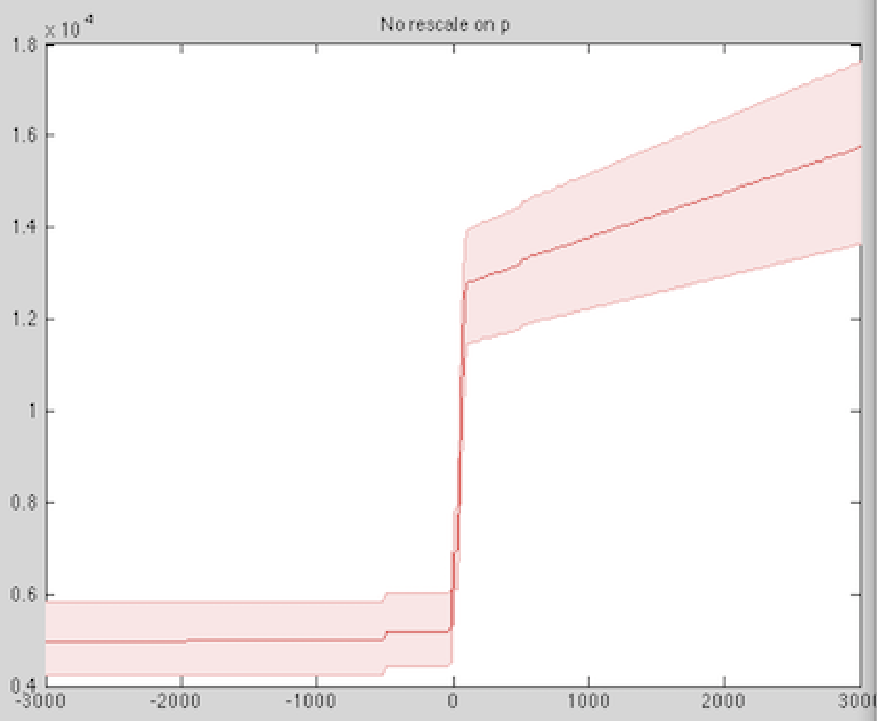
\includegraphics[trim=0cm 0cm 0cm 0cm, clip=true, height=50mm]{figch2/MC3.pdf} 
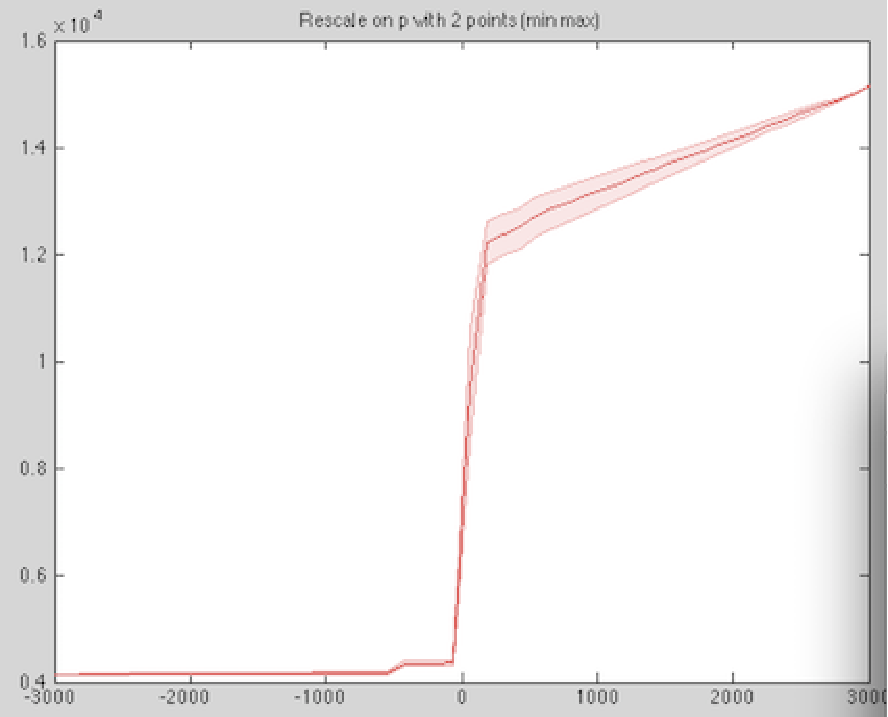
\includegraphics[trim=0cm 0cm 0cm 0cm, clip=true, height=50mm]{figch2/MC4.pdf} 
} \\
\makebox[\textwidth][c]{
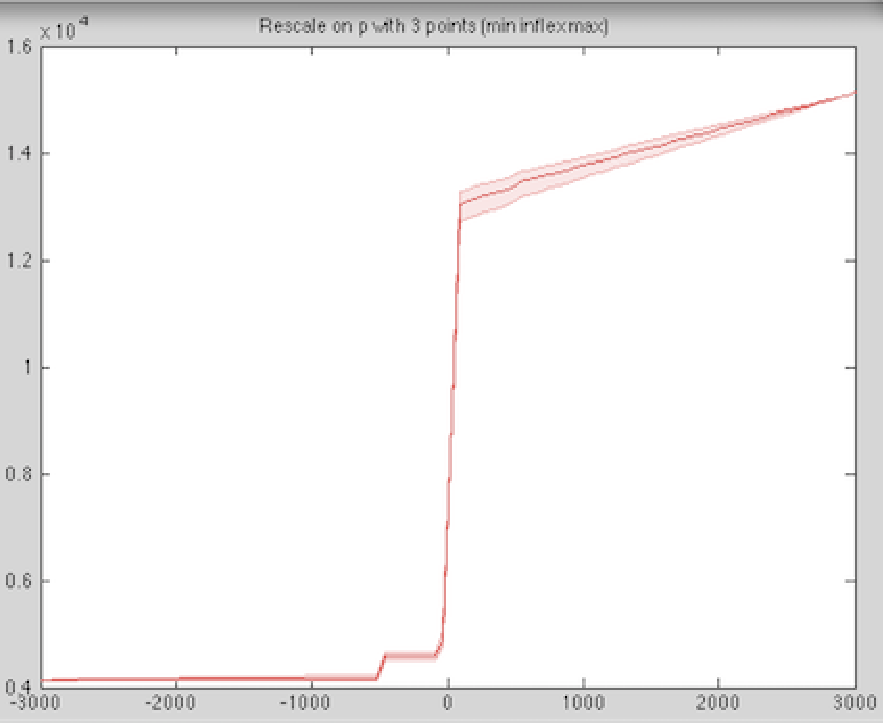
\includegraphics[trim=0cm 0cm 0cm 0.1cm, clip=true, height=50mm]{figch2/MC5.pdf} 
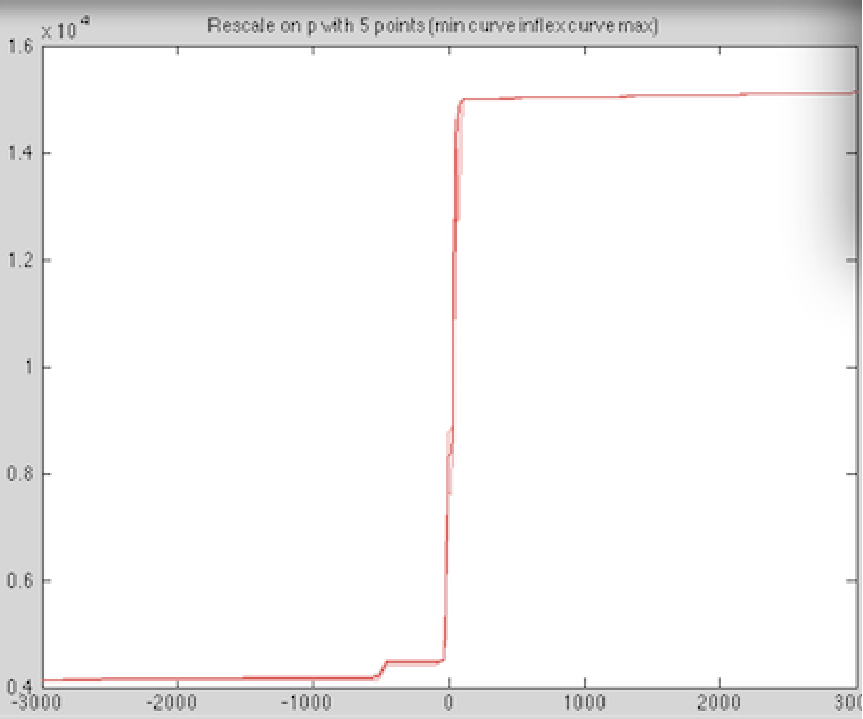
\includegraphics[trim=0cm 0cm 0cm 0.1cm, clip=true, height=50mm]{figch2/MC6.pdf} 
}
\caption{Error bars as a function of the number of extracted points}
\label{errorbarsasfunction}
\end{center}
{ \small Note: The graphs represent the master curve with the error interval for inferring the original bid function, conditional on the number of extracted, reference  points (RP). Top left (A): Computed without any RP. Top right (B): Computed using 2 RP. Bottom left (C): Computed using 3 RP. Bottom right (D): Computed using 5 RP. } 
\end{figure}

We can see that as we include an increasing number of points the shaded areas shrink : this is a measure of how much of the information contained in the raw curves is captured by the registration points. We see that at 5 registration points, the shaded area is very small, so much so that one can consider that by registering these 5 points, we capture a so-called "master curve" : most of the information about the curves is contained in those 5 points.\\

More quantitatively : without any reference point, inferred bid functions would lie in the interval shown in graph A of figure \ref{errorbarsasfunction}. With two reference points (namely the minimum an the maximum quantity), the uncertainty is reduced as shown by the smaller error interval in graph B. Graph C adds a third point (the inflection point) and Graph D adds another two points (the two points of maximum curvatures). Figure \ref{errorbarsasfunction} shows clearly that with an increasing number of reference points, we obtain a more precise information about the original bid function. We quantify the informational gain by measuring the pink shaded area in each graph A to D. The result is shown in figure \ref{decreasingdegreesoff} and reveals decreasing marginal information for each additional point. By selecting $K=5$ points, we are able to reduce the shaded area by a factor of about 50 when compared to figure A (see figure \ref{decreasingdegreesoff}). We see this insight as support for using $K=5$ points for further work. \\

\begin{figure}[!ht]
\begin{center}
\makebox[\textwidth][c]{
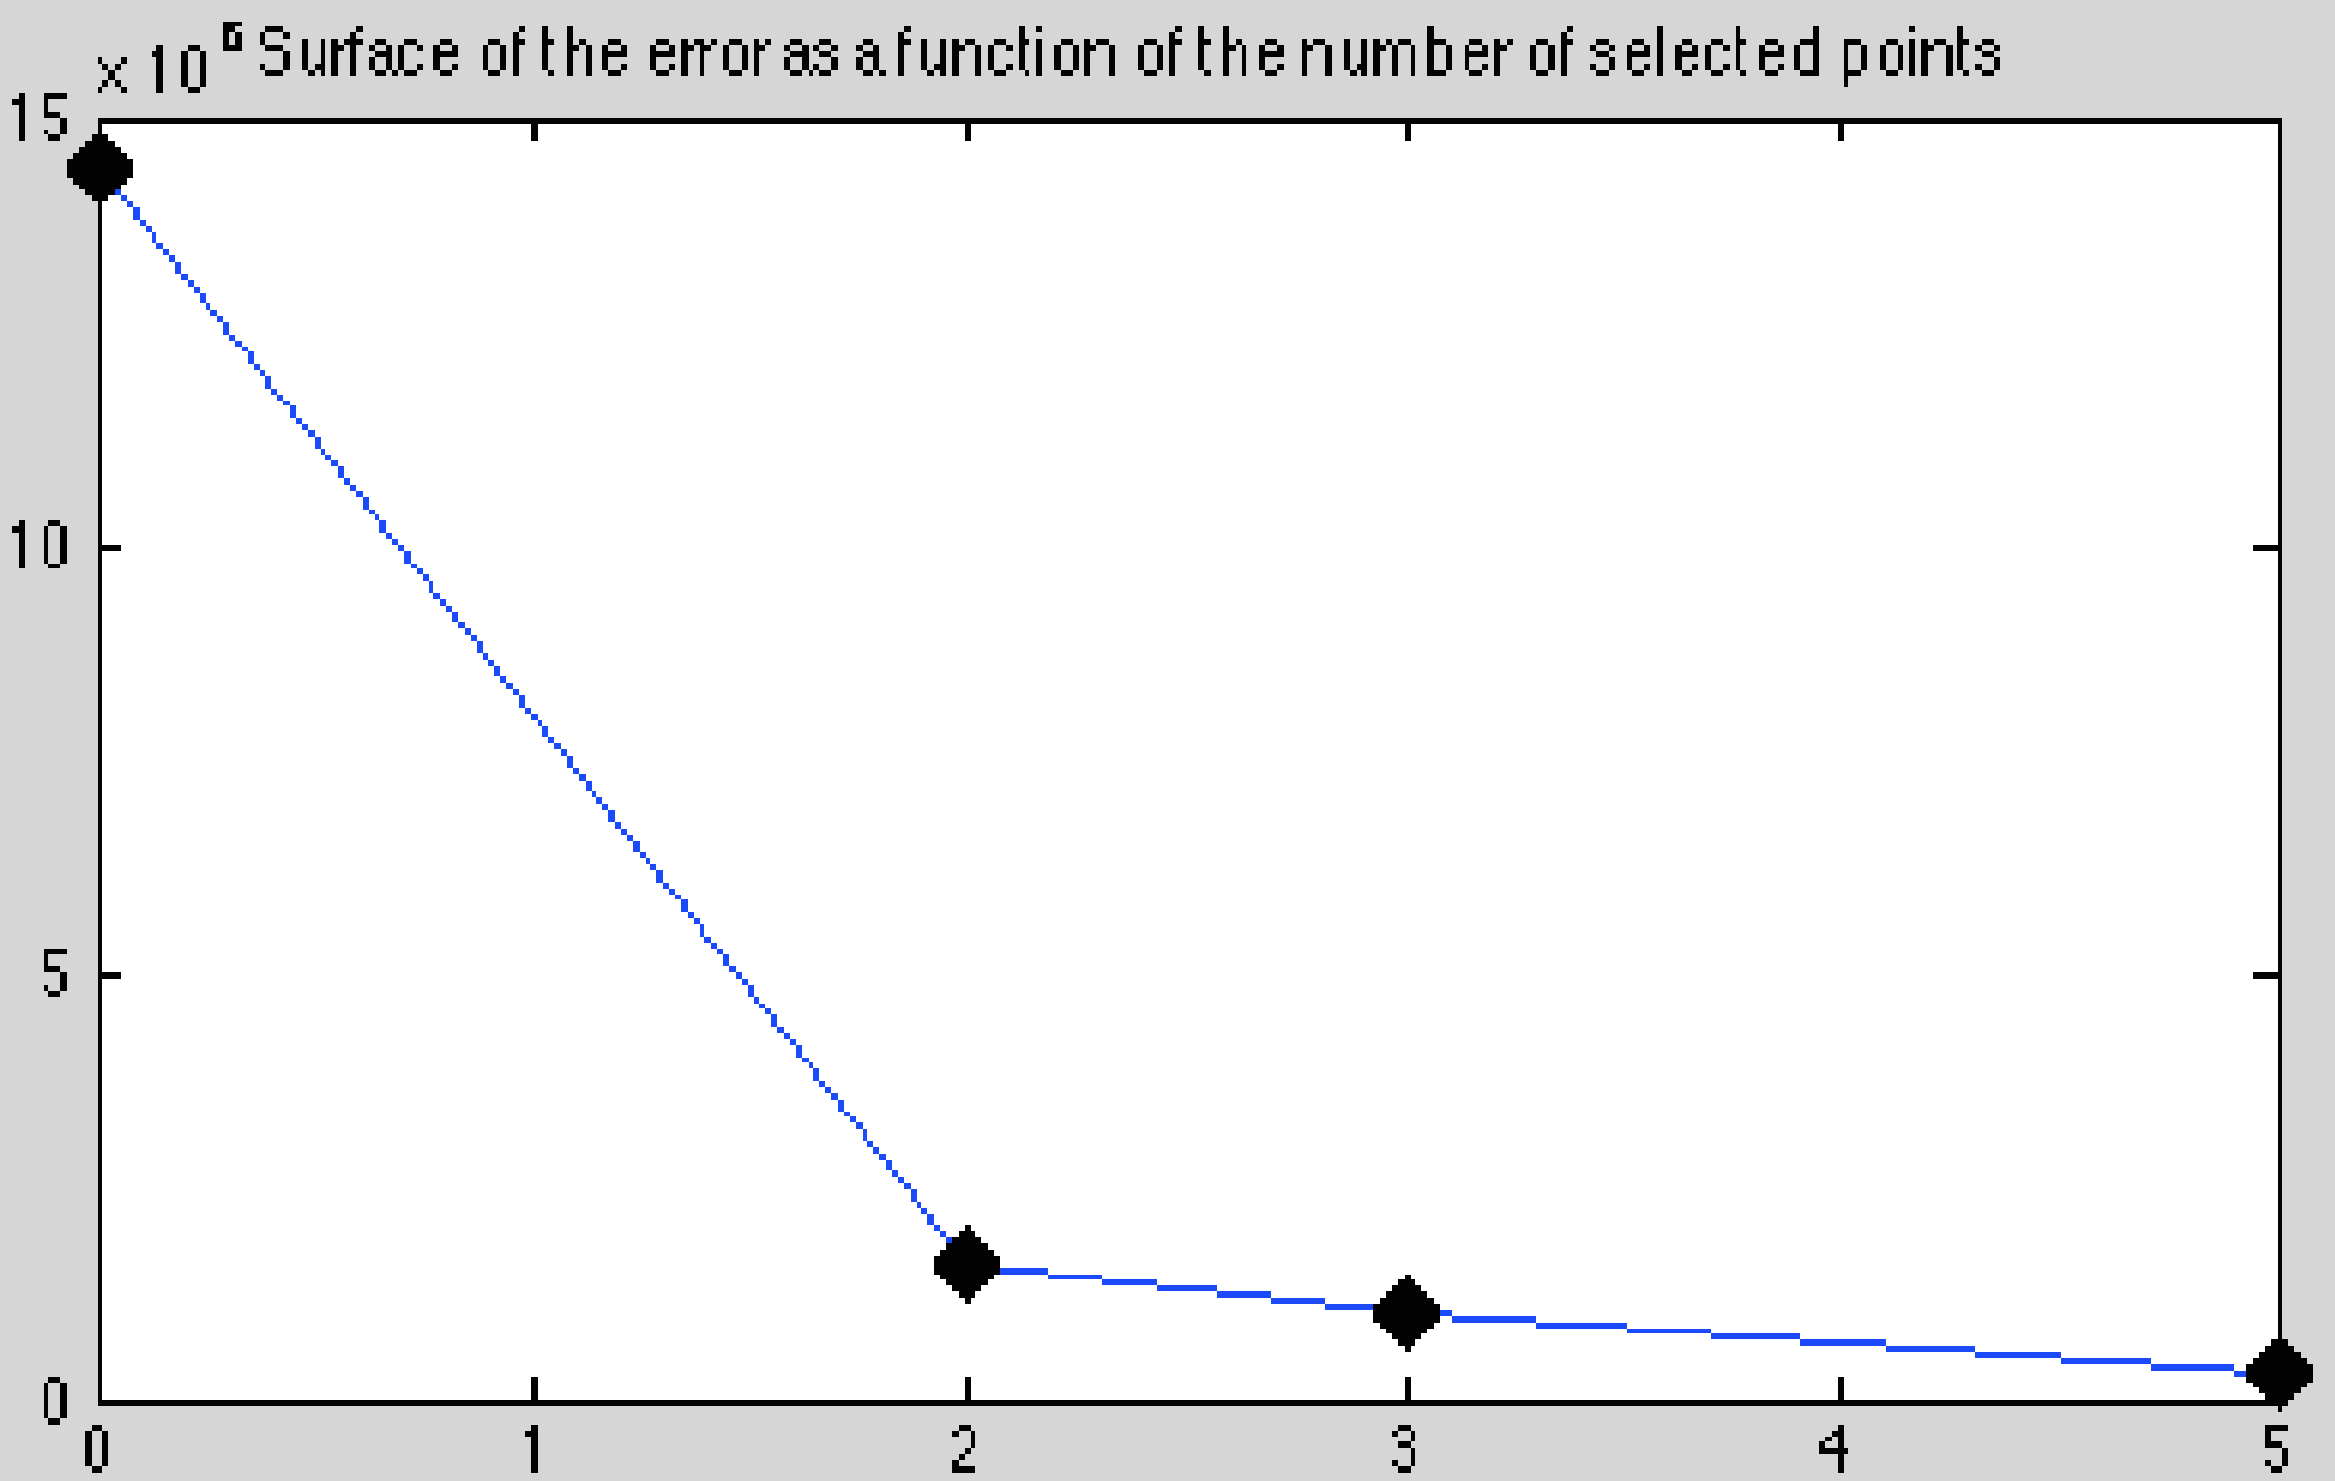
\includegraphics[trim=0cm 0cm 0cm 0cm, clip=true, height=50mm]{figch2/MC7.pdf}
}
\caption{Proxy for degrees of freedom on master curve}
\label{decreasingdegreesoff}
\end{center}
{ \small Note: The graph plots a proxy for the number of degrees of freedom for the inference of the original bid function on the number of reference points. Specifically, it plots the size of the pink shaded area in figure \ref{errorbarsasfunction} against the number of points. } 
\end{figure}

While the graphs in figure \ref{errorbarsasfunction} are displayed on inverted axes and rescaled units, we show the final master curve and uncertainty interval on the original axes and units in figure \ref{notrescaledmastercurves}. 

\begin{figure}[!ht]
\begin{center}
\makebox[\textwidth][c]{
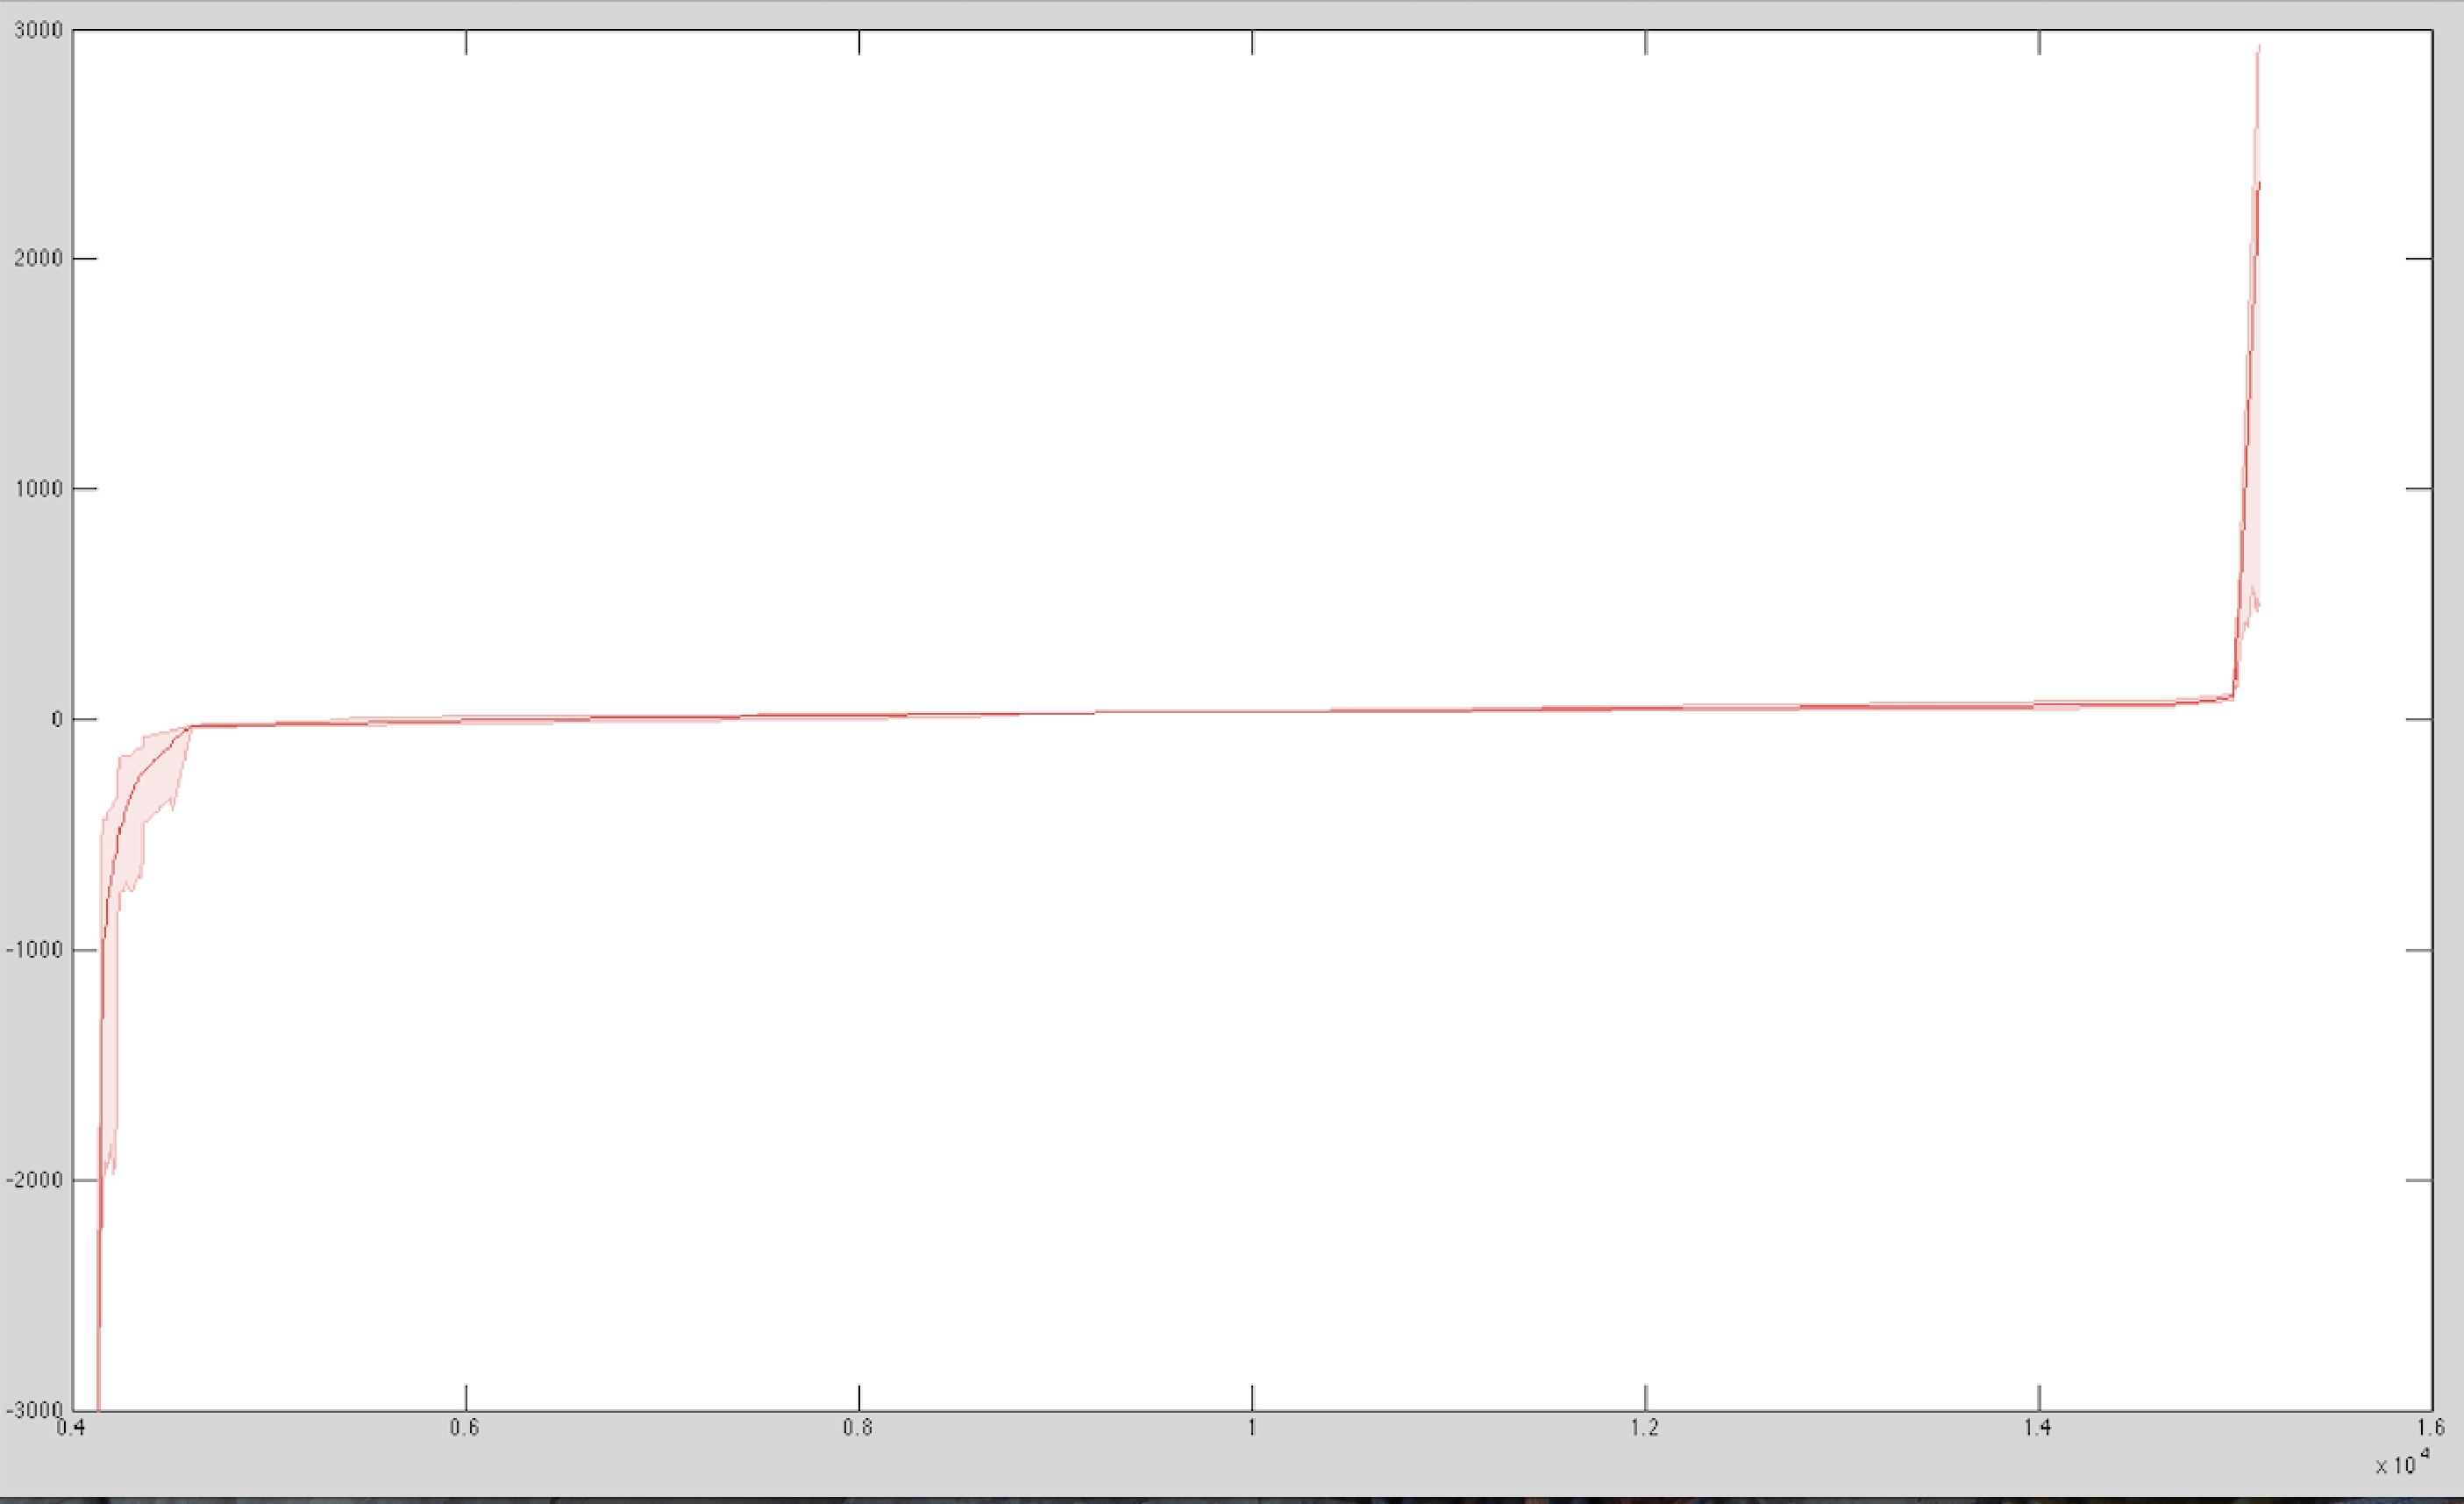
\includegraphics[trim=0cm 0cm 0cm 0cm, clip=true, height=45mm]{figch2/MC1.pdf}
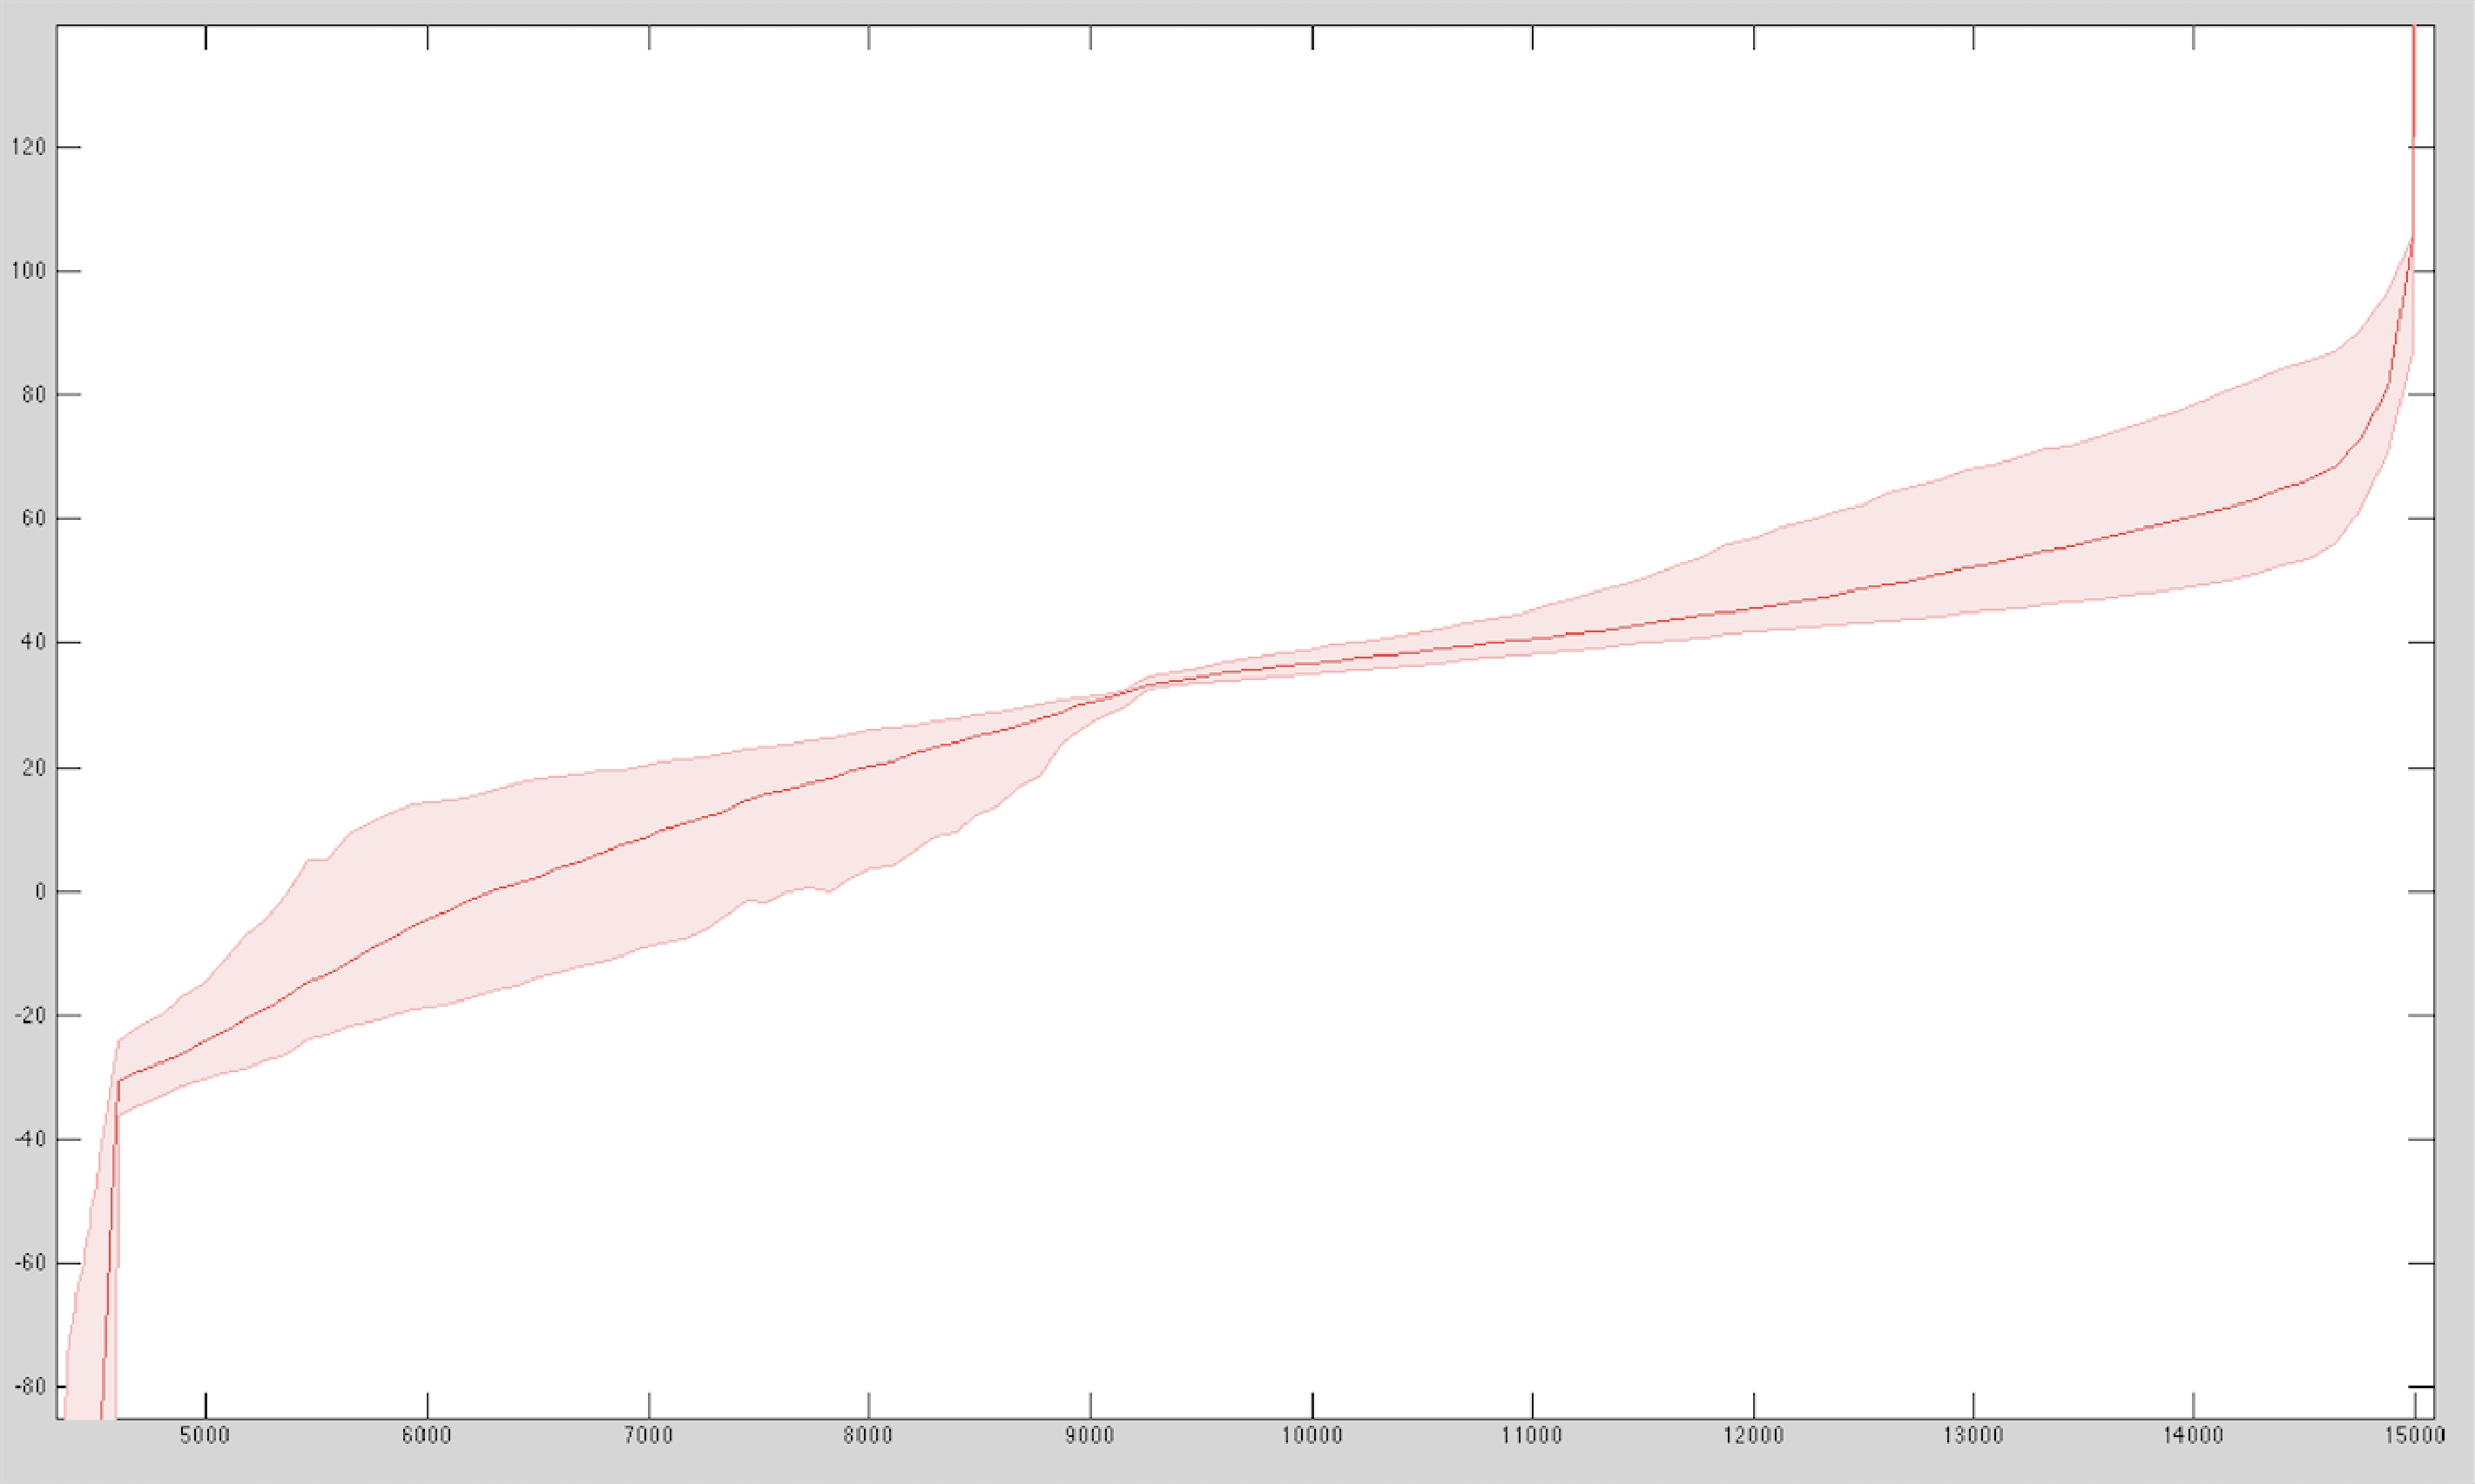
\includegraphics[trim=0cm 0cm 0cm 0cm, clip=true, height=45mm]{figch2/MC2.pdf}
}
\caption{Overall (left) and zoomed (right) Mastercurve with confidence interval}
\label{notrescaledmastercurves}
\end{center}
{ \small Note: Master curve in the quantity - price dimension.  } 
\end{figure}


\subsection{Discussion}
\label{pointccl}
In this section, we have developed an alternative technique to run a cross-section reduced form model on data generated by a market that keeps track of the full aggregate demand and/or supply functions. While we apply it to aggregate demand functions, the methodology is fit for the anaylsis of aggregate supply functions and individual bid functions of either market side.  \\

The methodology is inspired by the techniques used in the literature on Treasury auctions, but has been set up from scratch to allow treatment of more heterogenous data. Furthermore, the hard assumption of an underlying logistic function is relaxed and our non-parametric point selection avoids the storing of bid function information in the form of estimated function parameters, which are difficult to interpret. \\

Smoothing of the original bid functions is a component in both the traditional logistic function approach and our comparable point selection methodology. The smoothing enables the user to abstract of small bid function particularities and imprecision, e.g. steps in the function. However, in the traditional approach, the reduction of plus 1000 bid points into very few parameters resulted in the blurring of ``local" bid function information from all parts of the function at once. Our non-parametric approach allows specifically to control the extent to which one smoothes the underlying data through the amount of registration points considered.\\

The results of the comparable point selection are encouraging. We show that each type of point is distinctly chosen and that patterns of the original bid functions do not influence the quality of derivative information extracted at the selected points. We acknowledge the existence of bidding frictions in the original data and highlight this observation for further work. \\

\section{Methodology to aggregate geographically dispersed information on a national level}
The theoretical results of chapter 1 indicate that a key ingredient in explaining the dynamics of the bids submitted by suppliers on the electricity market is the uncertainty about demand shocks. \\

Energy  demand  addressed to the electricity markets depends on  temperature (through the heating of buildings), on wind speed (through the production of wind turbines which reduces the net demand) and on luminosity (through the production of solar panels which reduces the net demand). However, these three weather variables vary in space, whereas the market is at the national level. We introduce here the methodology with which we estimate the associated uncertainty.\\  

We have two types of meteorological data: observations and forecasts. We use both types of data to estimate the underlying uncertainty, the methodologies for each differ slightly. \\
\subsection{Dealing with meteorological data}
\subsubsection{Interpolation methodology on weather observations}
\label{interpmethodo}

Observations are obtained from M\'{e}t\'{e}oFrance for three parameters of particular interest: temperature, wind speed and light intensity. These observations take the form of tables of hourly observations for a given set of weather stations. Each parameter is observed on a different set of stations.\\ 

Due to their hourly nature, the analysis of the electricity market's sensitivity to weather requires a very high number of observations. Therefore we select between one and two stations per D\'{e}partement\footnote{There are 95 D\'{e}partement in France}, a French administrative unit of roughly 6000 $km^2$, i.e. of a typical lengthscale of about 75 $km$. We have 161 stations for temperature, 113 stations for wind speed and 106 for light intensity, as shown in Fig \ref{fig:stations}. \\


\begin{figure}[!ht]
\begin{center} 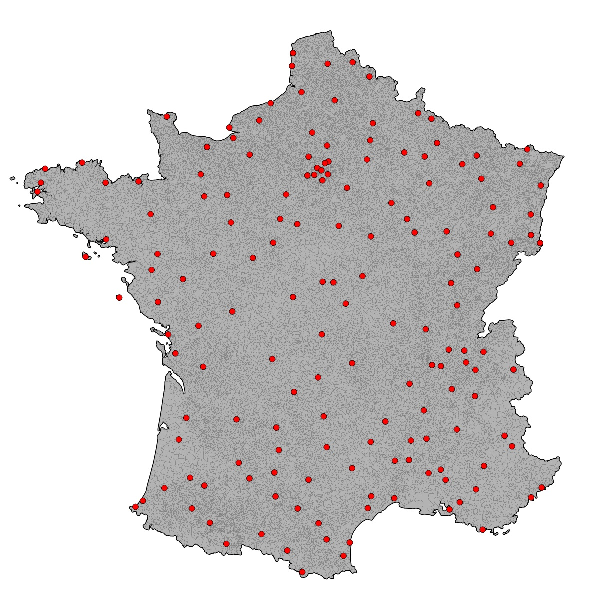
\includegraphics[height=45mm]{forqgis/stationstemp.pdf} \hspace{0.05cm}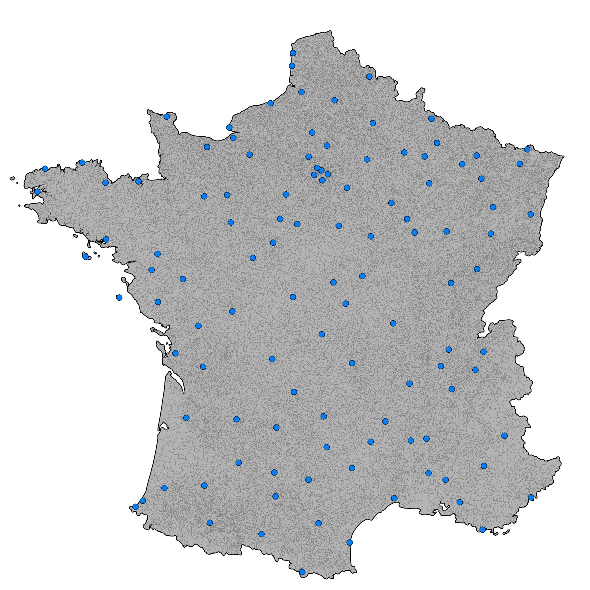
\includegraphics[height=45mm]{forqgis/stationswind.pdf}
\hspace{0.05cm}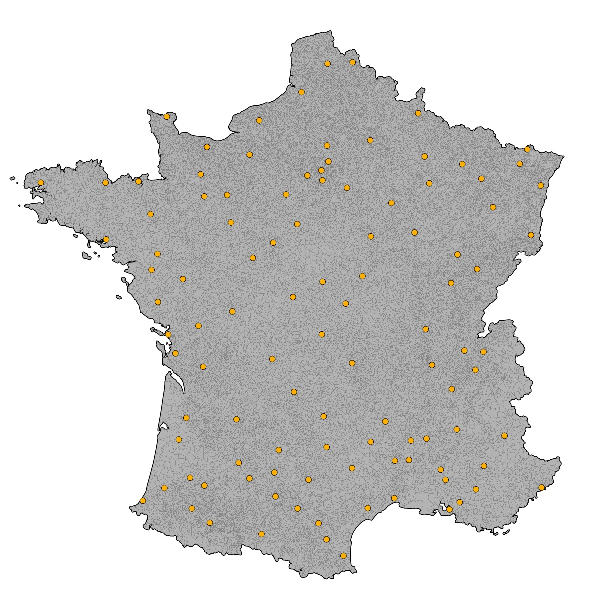
\includegraphics[height=45mm]{forqgis/stationslum.pdf}
 \end{center}
\caption{Stations for which we have hourly data. Left : temperature, center : wind speed, right : light intensity.}
\label{fig:stations}
\end{figure}

For each hour, we select the corresponding observations and interpolate them in order to reconstruct the weather on the entire french territory. An interpolation consists on inferring the value of a variable at query points using a reference data set of known values. One very important underlying assumption of interpolation methods is that of the continuity of the process underlying the data generation. The easiest interpolation method is the linear interpolation: think about a dataset of hourly observations with one missing value; to reconstruct the missing value, take the average of the value of the preceding and following hour. There are numerous methods of interpolation, even more so when the data is spatial in nature, all revolving around two main steps. First, given a query point at which one would like to infer the value of the variable, there needs to be a selection rule to know which of the points from the reference data set should be used (in our example the preceding and following values). Second, once these points are selected, one needs a weighting function to know their relative importance in order to obtain the interpolated value (in our example it is a simple averaging, that is weights of $0.5$). \\

We use the natural neighbor interpolation method, well known for its good balance between speed and accuracy. In short, in this case, the first step makes use of the Voronoi tessellation algorithm\footnote{The Voronoi tessellation algorithm takes a collection of points $\{p_k\}$ in the plane, and then partitions the plane as regions "belonging" to each point, called cells. A Voronoi cell associated with a given point $p_k$ is defined as the collection of every point in the plane whose distance to $p_k$ is less than or equal to its distance to any other $p_{-k}$. Each such cell is a convex polygon.}, one is able to define the natural neighbors of a point for which one seeks an interpolated value. These natural neighbors are used in the second step, which performs the actual interpolation as a weighted average of the values of these natural neighbors using a ratio of surfaces as weights (see Fig \ref{fig:natneighb} for more details).

\begin{figure}[!ht]
\begin{center} 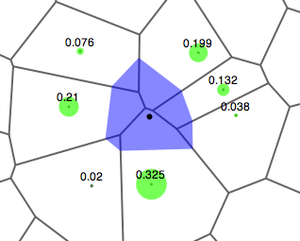
\includegraphics[height=27mm]{forqgis/natneiweights.png} \hspace{0.05cm}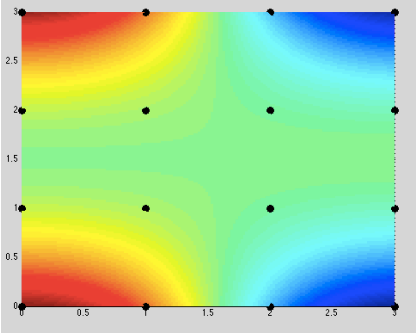
\includegraphics[height=27mm]{forqgis/natneiref.pdf}
\hspace{0.05cm}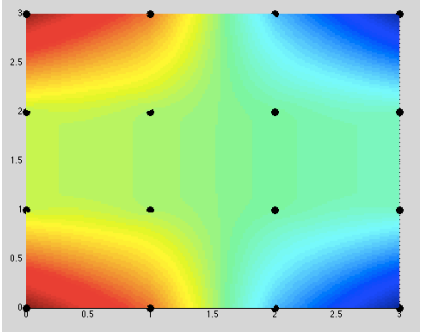
\includegraphics[height=27mm]{forqgis/natneireco1.pdf} \hspace{0.05cm}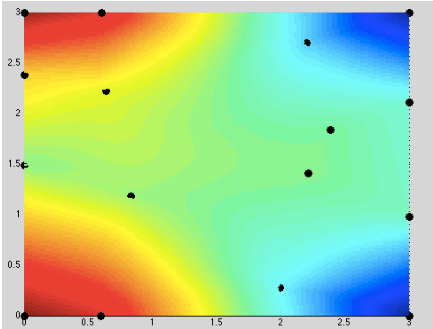
\includegraphics[height=27mm]{forqgis/natneireco2.pdf}
 \end{center}
\caption{\small Left: Voronoi's algorithm is applied once on the reference points highlighted in green to obtain the white surfaces, and a second time on the same points to which is added the query point in the center to obtain the new blue cell. The green circles, which represent the interpolating weights, are generated using the ratio of the shaded area to that of the cell area of the surrounding points. Center left: example of a reference surface (color mapped) to be reconstructed through a natural neighbor interpolation. Center right: interpolated surface with a reference set of 16 evenly organized points, represented in black. Right: interpolated surface with a reference set of 16 unevenly organized points, represented in black. From 16 points one is able to reconstruct the color mapped surfaces which are approximations of the reference one, represented in the center left image. }
\label{fig:natneighb}
\end{figure}


\subsubsection{Image transformation to recover weather forecasts}
\label{picturemethodo}

Forecasts are obtained from the Global Forecast System (GFS), and come in the form of colormaps, as shown in Fig \ref{fig:refmeteociel}. We are going to illustrate our methodology on temperature data, but the same exact approach is performed on wind speed data. The general idea is that the pointwise precision is low (2$^{\circ}C$ per color) but that the overall map contains quite a lot of information through the topology of the colored regions. We describe below how to extract this information. 
 
\begin{figure}[!ht]
\begin{center} 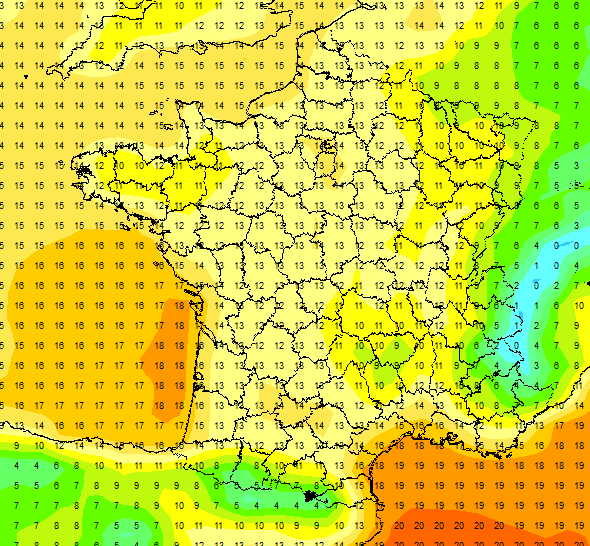
\includegraphics[height=60mm]{forqgis/ref-2011-11-03-15.png}
\end{center}
\caption{\small Temperature forecast from a simulation run by the GFS at 6 a.m. on the 3rd of november 2011, for a forecast at 22 p.m. }
\label{fig:refmeteociel}
\end{figure}

\subparagraph{First: image cleaning} To extract the relevant data we first clean the color map from its irrelevant information, namely the temperature in numbers and the administrative borders. Note that this step introduces a small amount of high spatial frequency noise, see Fig \ref{fig:mciel} left and center left. 

\subparagraph{Second: removal of redundant information} A lot of information is lost from the actual GFS simulations by using a color map representation, as temperature is described as a discontinuous variable: each color has a precision of 2$^{\circ}C$. In order to correct for this, we leverage the fact that all the information contained in this color map, that is the color at each pixel, is actually contained in a smaller set of points. Consider the value at the boundaries between different color regions: by knowing that the interior of a constant color region has a constant value, one is able to represent all the information contained in the original image by keeping only track of the values at the boundaries. To recognise those boundaries we perform image analysis, more precisely we use edge recognition methods based on finding high gradient regions, thus obtaining Fig \ref{fig:mciel} center right. 

\subparagraph{Third: surface fitting} Once we represent the information in this denser form we can perform the last step, which consists in fitting a surface to our newly defined dataset, i.e. the temperature values at the boundaries, which take the form of $(x,y,T)$ triplets. We could perform an interpolation, but these methods are not well suited to reference sets having so much structure. Here, data points lie on curves representing iso-temperatures, so that along such a curve there is a lot of data points, whereas the information is very sparse along the direction of the gradient. In addition the first step introduced some spatial noise which we want to correct to some extent : we allow our fitted surface to take different values than our data points, so as to smoothen out this noise. We define the rigidity of our fitted surface, i.e. a penalty associated to fast changes in the value of the surface, and therefore reduce the importance of the high frequency noise introduced in the first step. The end result is presented in Fig \ref{fig:mciel} right. \\

It is key to understand that this image is displayed using a colormap close to the one in the original picture to facilitate comparison but that its underlying data is continuous whereas the original image describes temperature by bins of 2$^{\circ}C$. It can therefore be used to query the value at any given point, and these values will change continuously in space instead of discrete jumps in the raw format.\\

\begin{figure}[!ht]
\begin{center} 
\makebox[\textwidth]{
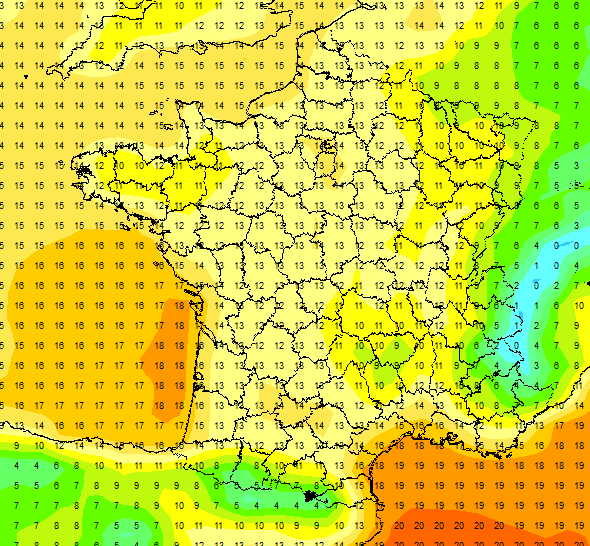
\includegraphics[height=30mm]{forqgis/ref-2011-11-03-15.png} \hspace{0.05cm}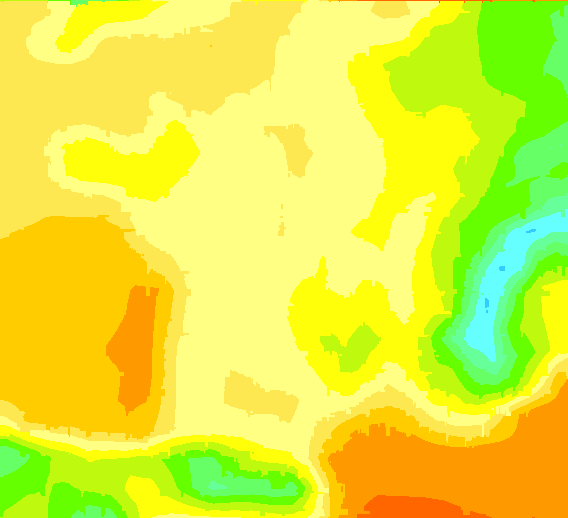
\includegraphics[height=30mm]{forqgis/2011-11-03-15.png}
\hspace{0.05cm}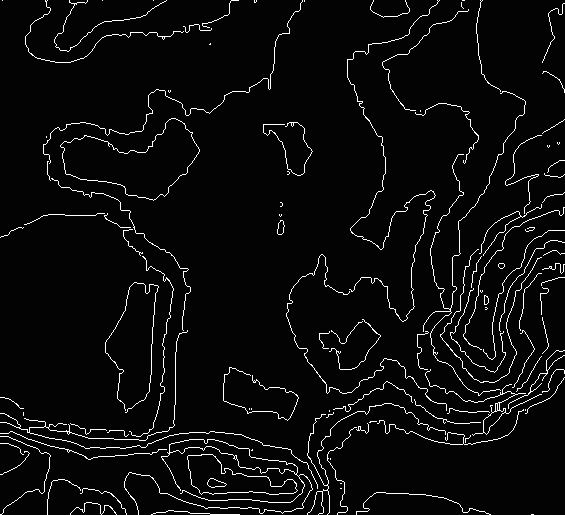
\includegraphics[height=30mm]{forqgis/mcieledge.png} \hspace{0.05cm}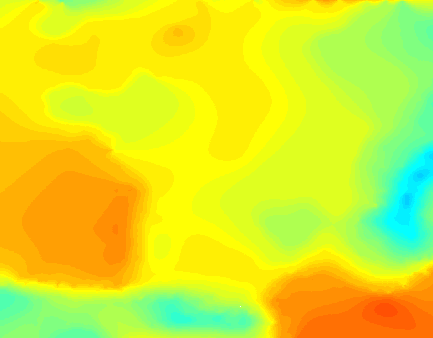
\includegraphics[height=30mm]{forqgis/mcielsmooth.png}
} \end{center}
\caption{\small Left: reference image. Center left: borders and numbers are removed. Center right: edge recognition. Right: final fitted surface. }
\label{fig:mciel}
\end{figure}

\subsubsection{Autocorrelation lengthscale}
\label{autocorr}
We use this dataset to build measures of the weather uncertainty. To do so we measure the auto-correlation lengthscale of our three weather variables of interest : temperature, wind speed and light intensity. This lengthscale measures how much are the weather variables correlated spatially. Our hypothesis is that the auto-correlation lengthscale is inversely proportional to uncertainty about the variable we are interested in. When it is small, the variable is less spatially correlated, which we interpret as being more difficult to forecast. Conversely, when the auto-correlation lengthscale is large, the variable is very correlated spatially, that is that the informational content of one datapoint is higher for the prospect of using it for the evaluation of a national effect.\\

More precisely, the argument is as follows: \\
\textbf{First}, renewable production is built by aggregating the forecast of all individual renewable sources. This means knowing the position and capacity of every renewable source, querying weather forecasts for all of these points, modeling the renewable's response to the forecasted weather, and adding the forecasted productions. \\
\textbf{Second}, we note that weather is spatially correlated, which means that the closer two points are, the closer the values for a given weather variable (the air temperature at your left hand is very close to that at your left hand, but less so across the city, and even less so across the country). This correlation roughly follows an exponential law : the difference between the values of a weather variable between two points behaves in a linear fashion for small distances, and saturates at large distances \footnote{Intuitively, the characteristic lengthscale of autocorrelation represents the distance required between two geographical points on a map of weather forecasts to observe a decorrelation of half of its maximum value. For example on the wind speeds prediction, a characteristic length of 80 km means that if we observe two very distant points (say 1000km) to have a difference in wind speeds of, on average, 50km/h (this being the maximum difference, we are in the saturated regime), then we will observe, on average, wind speed differences of 25km/h for points distant from each other by 80km.}. The transition between those two regimes is given by a caracteristic lengthscale, a bit less than 200km on average. \\
\textbf{Third}, we observe that the average distance between production points is large enough that the relevant regime of autocorrelation is the saturated part \footnote{For N production points, we compute the N(N-1)/2 pairs of points, consider their distances, and compute the average of these distances weighted by the production capacity at every point. In the case of the wind we have an average distance of 459 km, in the case of the photovoltaic production we have an average distance of 499km.}. \\
\textbf{Fourth}, we note that there are two main channels through which the overall uncertainty about renewable production is related to the weather. There is an issue of error averaging, which means that if the weather becomes very spatially uncorrelated, one can expect errors to cancel out relative to a given bias in the forecast. This channel would tend to imply that more spatial variations imply a smaller uncertainty about production. There is also the issue that weather forecasts are numerical simulations and that the mesh size for such simulations, typically 5km for the high precision ARPEGE model of Météo France, implies that the errors are higher as the simulated phenomenons have higher gradients. This means in our case that the uncertainty about the forecast increases as the weather becomes more spatially uncorrelated. \\
\textbf{Fifth}, these two effects are of opposite signs, but our third point is an argument for considering that the averaging of errors is smaller than the simulation errors. Therefore we expect our uncertainty to increase as the spatial autocorrelation decreases (i.e. more spatial variation). \\

This can be summed up with the following hand-waving argument : when there is more spatial variations, the weather is more messy, therefore more difficult to predict. \\

To understand what the autocorrelation lengthscale captures, take two points on a plane and a spatially correlated bounded variable. If those points are infinitely distant, the value of the variable at these points should be uncorrelated. That is that the absolute difference between the variable taken at those two points should have a given average value. Conversely, two points infinitely close should have the same value, i.e. a zero absolute difference between the variable taken at those two points. The question is how fast is the transition between those two limit cases. First, we define the average absolute difference between two points when distant of a given value. Second we extract a typical lengthscale. \\

To define the average absolute difference between two points when distant of a given value, we consider at a given point in time every possible pair of points in our dataset. For a given pair we compute its distance and its absolute difference in value (in black in Fig.\ref{figautocorrel}). For 100 datapoints we obtain 4950 pairs. We then use a kernel smoother in order to obtain the average non parametric autocorrelation function (in blue in Fig.\ref{figautocorrel}). \\

To recover a typical lengthscale we make the parametric assumption that the auto-correlation is exponential in nature. We fit an exponential function through our smoothed data (in red in Fig.\ref{figautocorrel}), and recover the exponential decay parameter as our lengthscale (in green in Fig.\ref{figautocorrel}). We perform this operation for every hour in our dataset and every weather variable. The results are timeseries for the characteristic lengthscale of the weather parameters.


\begin{figure}[!ht]
\begin{center} 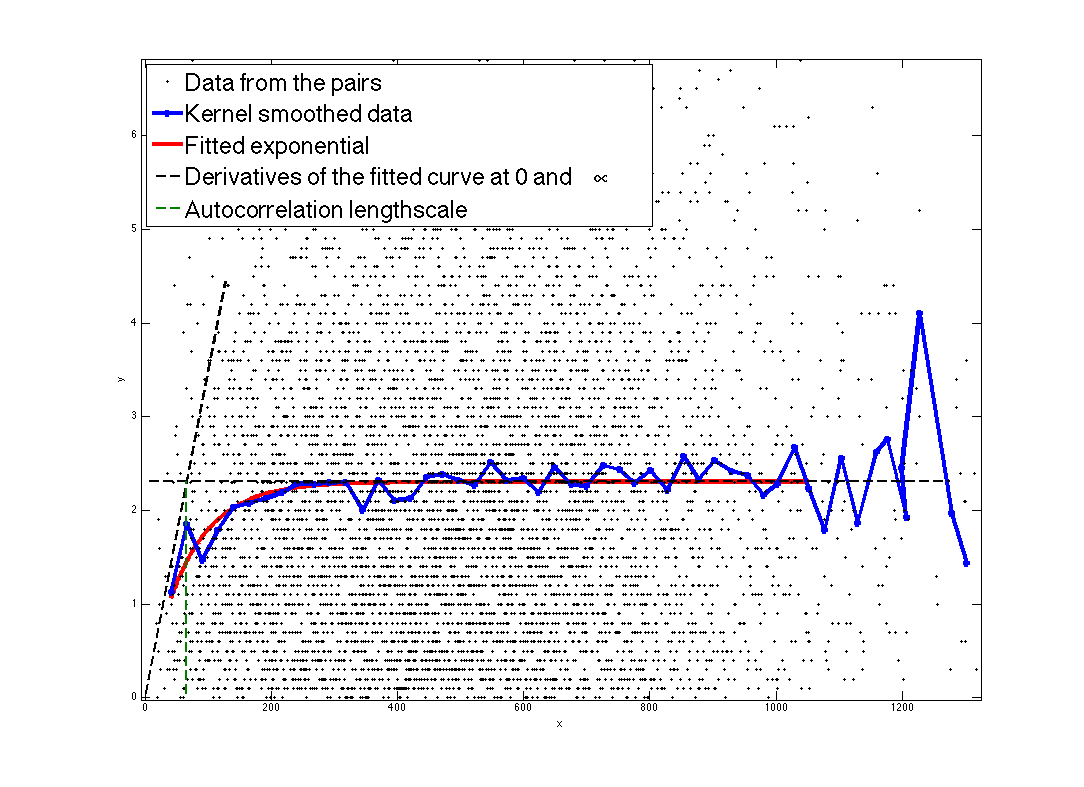
\includegraphics[height=95mm]{forqgis/lautocorgraph.png}
\end{center}\vspace{-0.9cm}
\caption{Auto-correlation lengthscale computation. In black are the points obtained from all the pairs from our original data, that is absolute wind speed differences as a function of the distance between the two points. In blue is the kernel smoothed function from those points. In red is the exponential fit. In black are the derivatives of the fit at $0$ and $\infty$. In green is the recovered auto-correlation lengthscale. The unit for the lengthscale is in km.}
\label{figautocorrel}
\end{figure}

\subsection{Aggregation of local information}
\subparagraph{Wind1DA}
\label{Wind1DA}

\textit{Wind speed (average speed in km/h):} 
\label{winddetail}
Wind speeds influence the productivity of wind turbines, which are a source of unreliable electricity generation. In general, renewable technologies benefit from a feed-in guarantee by the state. That is, regardless of the trading outcome on all markets, renewable energies will be the first to be fed into the power grid at a guaranteed price. \\

Consequently, the electricity production of renewable technologies represents a production shock for all actors on the market. The production shock means that the demand to be served by traditional electricity producing firms is reduced by the amount that is serviced by the electricity gained from renewable sources. \\

In the case of wind turbines, the average speed of the wind per hour allows to proxy for the size of the production shock due to the electricity generation from wind energy. \\

We use hourly windspeed forecast in the form of color maps from the Global Forecast System (GFS), giving the speed by bin of 5 km/h at 10m above ground, and the location and production capacity of the wind turbines present on the french territory, given by the SOeS (service d'observations et d'études statistiques - observations and study department) a department of the french environment ministry. \\

We consider that all turbines in France are of the same type, that is that they have the same response curve and height. \\

A typical response curve is represented in Fig. \ref{fig:typpowercurve}. It has three main characteritics : the wind speed at which the turbine starts to produce electricity, called the cut-in speed, the speed at which the turbine reaches its rated output, called the rated ouput speed, and the speed at which the turbine has to stop to avoid damage, called the cut-out speed. We use data publicly available\footnote{http://www.thewindpower.net } to obtain a rough estimate of the french average wind turbine characteristics. We use a cut-in speed of 2.5 m/s, a rated output speed of 14 m/s, and reduce arbitrarily the cut-out speed from an estimate of 24 m/s to 20 m/s to account for the fact that a turbine is shut down not when the average speed is too high but when the maximal speed becomes dangerous for the turbine.\\ 

Wind speed also increases with height, and turbines are typically between 60 and 80m high. We therefore apply a multiplier to the reconstructed wind speed at 10m. \\

We seek to reconstruct the french wind energy production from meteorological data. The two adjusted values, the cut-out speed and the speed multiplier, are adjusted by hand to obtain reasonnable fits. The reason for this is that the reconstruction of wind speed and aggregate production is computationnally intensive, therefore we cannot perform a full blown estimation. We choose these values with a precision of roughly 10\% with repect to their admissible range of values. \\

\begin{figure}[!ht]
\begin{center} 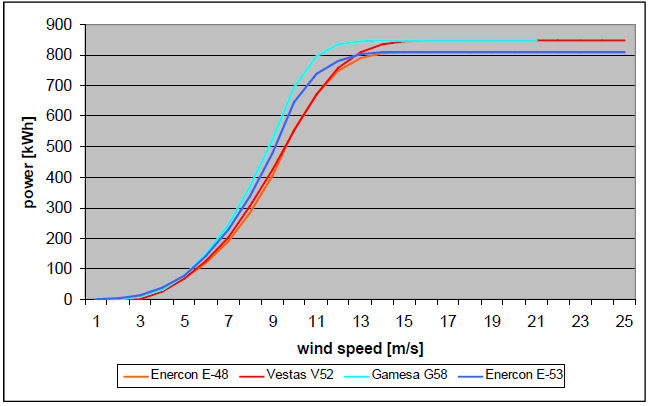
\includegraphics[height=50mm]{forqgis/ref-powercurve.png}
\end{center}
\caption{\small Typical response curves of different wind turbines}
\label{fig:typpowercurve}
\end{figure}


We obtain a reconstruction of wind production from day-ahead wind speed forecasts that we compare to actual observed production and to day-ahead wind production forecast computed by RTE, the french grid operator as shown in Fig.\ref{fig:windreco1DA}. We stress here that our aim is two-fold: to link wind turbines' production to weather data and to use forecast data as the market actors only possess this information when bidding. We do not aim at producing better forecasts than the grid operator, the figure is only displayed to show that our methodology produces reasonable estimates (we obtain a correlation coefficient between our forecast and the observation of $0.85$ where the grid operator obtains $0.97$).  

\begin{figure}[!ht]
\begin{center} 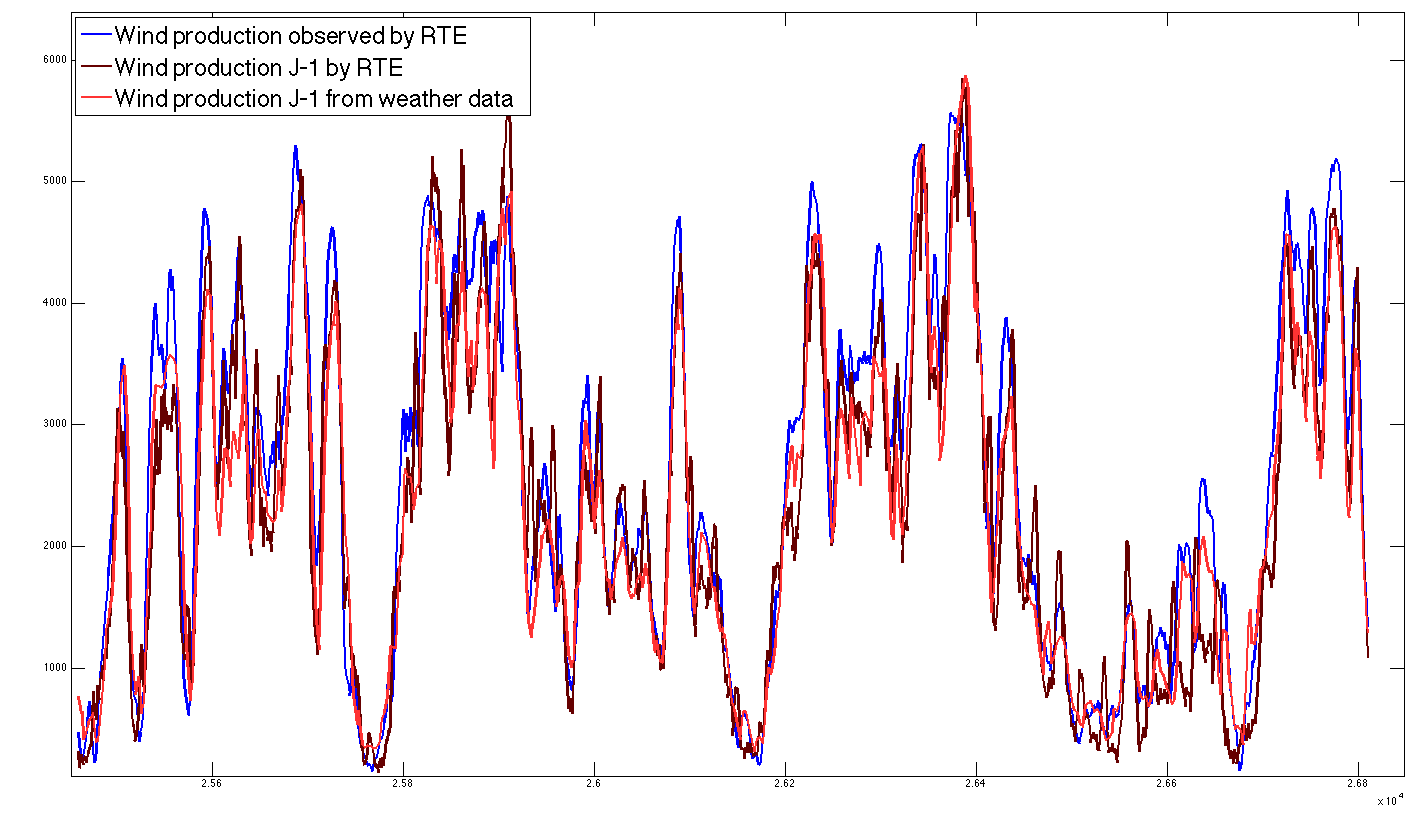
\includegraphics[height=80mm]{forqgis/windprodD1A.png}
\end{center}
\caption{\small All curves are hourly production data. The origin of the hours is the first of January 2011, and the production is in MWh. In blue: the observed wind production. In dark red: the day-ahead predictions from the grid operator. In light red: the day-ahead predictions from weather data.}
\label{fig:windreco1DA}
\end{figure}


\subparagraph{Tempeff15}
\label{Tempeff15}

We focus on the effect of temperature on the demand of electricity first. In France, a high percentage of the population heats their housing with electricity, therefore cold waves have a high impact on electricity consumption: 2300MW of additional power consumption for every drop of 1$^\text{o}C$ below 15$^\text{o}C$, as shown in Fig.\ref{elecconstemp} sourced from \cite{rtewebsite1}, the French grid operator. \\

\begin{figure}[!ht]
\centering
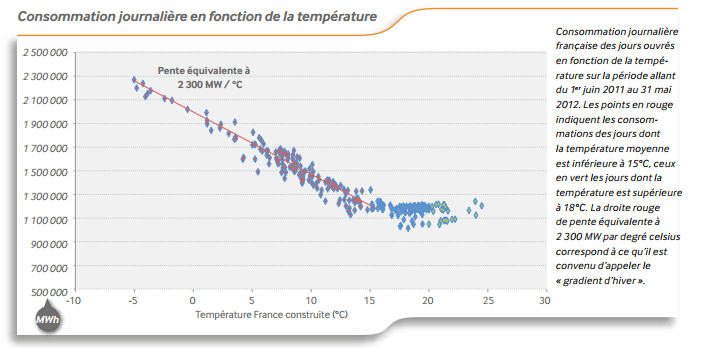
\includegraphics[height=65mm]{forqgis/Temp_Cons_France_RTE.png} 
\caption{Daily electricity consumption in France as a function of the temperature}
\label{elecconstemp}
\end{figure}


We apply this information to our observed meteorological data in order to build an effective temperature for France aimed at capturing its effect on consumption. To do so, we reconstruct temperature data for every french \emph{commune}, the smallest administrative unit in France (there are around 36000 of those). We consider population as being a good proxy for potential heat consumption, therefore we apply it as a weight to the \emph{commune} temperature. Lastly, we consider that temperatures saturate at $15^\text{o}$C. This allows us to build an effective temperature taking into account where the population is located and the nonlinearity of heat start up which in turn allows us to account at the country-level for the local impact of temperature on the electricity consumption.  \\

\subparagraph{Solar}
\label{Solar}

Light intensity (in $W.m^{-2}$) impacts the electricity market through multiple channels. The most obvious one is the associated electric production from photovoltaic panels. But there is another channel through which lighting can be seen as impacting electricity consumption : more sunlight decreases artificial light usage. In France, annually, the electric consumption that can be attributed to lighting represents roughly 50 TWh where solar production is roughly 4 TWh\footnote{These estimates are computed by the authors based on numbers coming from \cite{eleceurope}, INSEE and EDF}. \\

We have photovoltaic production data, which in itself is a blackbox. As we aim to link meteorological data to consumption we first want to validate the quality of our meteorological data. To do so we reconstruct the photovoltaic production from weather data. We know what are the hourly luminosity conditions on the french territory but also where is installed the photovoltaic production capacity. The SOeS (statistical observation and study department), a branch of government, publishes each year a file containing the installed capacity of renewable energy sources per communes, a french administrative unit with a typical size of roughly 3 $km$. \\

We use observed luminosity data from M\'{e}t\'{e}oFrance, as there is no hourly forecast of luminosity, and assume a sigmoid response from photovoltaic panels to light intensity with a saturation towards high light intensity, that is approximately a linear response up to a certain threshold. The results are shown in Fig.\ref{solarreco}.  \\

\begin{figure}[!ht]
\centering
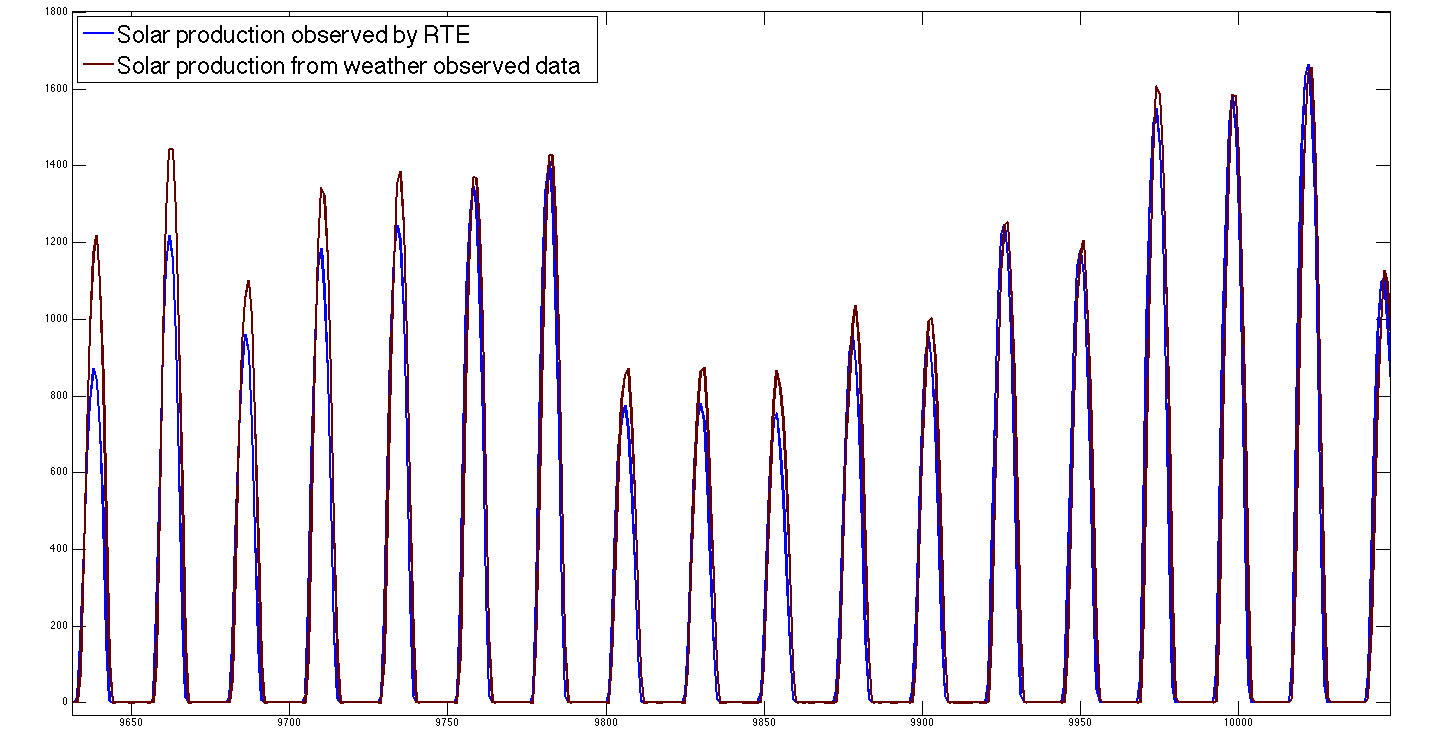
\includegraphics[height=65mm]{forqgis/solobs_reco.png} 
\caption{Hourly solar production in MWh. The time origin is the first January 2011. In blue: observed production by RTE. In dark red: reconstructed production from observed weather data.}
\label{solarreco}
\end{figure}


We observe that solar production is much more regular than wind production, therefore it is not possible to build a proxy for lighting consumption that would allow us to decorrelate the effects from production and lighting. We therefore stick to this proxy to capture the net effect of both channels.

\subsubsection{Other controls}
\subparagraph{Tempeff}
We also build an effective temperature that does not account for the nonlinearity at $15^\text{o}$C following the same methodolgy otherwise as a control. 


\subparagraph{Roll\_Temp$H$}
\label{rolltemp720}
Variable capturing seasonal trends by using the rolling average temperature on effective temperature (Tempeff15) over the last $H$ hours, i.e. the last $H/24$ days. 

\subparagraph{Roll$_{avgTH}$} Variable capturing seasonal trends by using the rolling average temperature on temperature Tempeff (no kink) over the last H hours, i.e. the last H/24 days.

\subparagraph{suncycle}\label{suncycle} Variable capturing intraday seasonality be measuring the intensity of sun- light as a percentage of the maximum daily observation. Midday is defined at the maximum sun intensity every day, i.e. Midday = max(Solar). Thus, suncycle$_H$ = Solar$_H$ / Midday.

\subparagraph{deltasun}\label{deltasun} Variable computed to proxy for dusk and dawn. It is computed as the absolute difference between suncycle$_H$ - suncycle$_{H−1}$.

\subparagraph{SolarRest}
\label{SolarRest}
Solar represents estimates of solar production. Therefore, it is highly collinear to the daily suncycle variable since solar production is light dependent. %Furthermore, the sun is closer to the French earth in summer, thus it is also correlated to seasonal trends represented by Roll\_Temp720. 
SolarRest is the residual from a regression of Solar on suncycle %and IT1, where IT1 is an interaction variable of suncycle and Roll\_Temp720. 
and captures the unexplained part of solar production on top of pure light intensity considerations. Table~\ref{SolarBlack} gives the results of the regression.
\begin{table}[H]
\begin{center}
\begin{tabular}{lcc} 
%\toprule
 & (1) &  \\
% & Black\_3 &  \\
\textcolor{white}{VARIABLES} & Solar & SE \\ \midrule
\vspace{4pt} & \begin{footnotesize}\end{footnotesize} & \begin{footnotesize}\end{footnotesize} \\
suncycle & 1,500*** & 3.903 \\
Constant & 0.876** & 0.383 \\
%\vspace{4pt} & \begin{footnotesize}\end{footnotesize} & \begin{footnotesize}\end{footnotesize} \\
\midrule Observations & 150,959 &  \\
 $R^2$ & 0.702 &  \\ \bottomrule
\multicolumn{3}{c}{\begin{footnotesize} *** p$<$0.01, ** p$<$0.05, * p$<$0.1\end{footnotesize}} \\
\end{tabular}
\end{center}

\caption{\label{SolarBlack} Regression of Solar on suncycle}
%\emph{Note}: ****TBC
\end{table}

\subparagraph{RteBlackBox}
\label{RteBlackBox}
%\subparagraph{RTE's one day ahead prediction of total consumption:} 
RTE, the French grid operator gives day ahead predictions of the total hourly consumption, which are available at the time of bidding. This variable is called PrevConsoH. \\

We do not have access to the exact definition of the index and it is thus a black box. However, it is available to the firms at the time of bidding and we want to include it in the demand estimations. \\

At the same time, it is evident that the Index uses much of the information that we explicitly control for in the regressions, therefore collinearity is an issue. In order to have correct coefficient estimates, we adopt an instrumental variable approach by regressing the RTE prediction on our exogenous factors, extracting the residuals and only including the unexplainable component of the RTE prediction in the demand estimation in the form of a separate variable called RteBlackBox.\\

Formally, RteBlackBox is equal to the predicted residuals ($u$) of the following regression, where $X$ stands for the vector of explanatory variables: Tempeff15,  Roll\_Temp24 ,  Roll\_Temp240, suncycle, morning, deltasun and EWH.  \\
\begin{equation}
\label{blackreg}
 \text{PrevConsoH} = a + bX +u 
\end{equation}
In table \ref{black1} we give the output of regression \ref{blackreg} in column $1$, which is strong support that our prepared data for exogenous variables is of very high quality. We highlight the significance of all explanatory variables at the $1\%$ level and the R$^2$ statistic of $85.3\%$. \\

\begin{table}[!ht]
\begin{center}
\begin{tabular}{lcc} \toprule
 & (1) & (2) \\
% & Black\_1 & Black\_1 \\
\textcolor{white}{VARIABLES} & PrevConsoH & PrevConsoH \\ \midrule
%\vspace{4pt} & \begin{footnotesize}\end{footnotesize} & \begin{footnotesize}\end{footnotesize} \\
Tempeff15 & -682.6*** &  \\
Roll\_Temp24 & -802.0*** &  \\
Roll\_Temp240 & -1,175*** &  \\
SolarRest & -0.860*** & -0.345*** \\
suncycle & 7,849*** & 7,418*** \\
morning & -4,759*** & -4,398*** \\
deltasun & 10,108*** & 9,010*** \\
EWH & -1,245*** & -1,254*** \\
Tempeff &  & -301.4*** \\
Roll\_avgT24 &  & -687.3*** \\
Roll\_avgT240 &  & -918.2*** \\
Constant & 77,701*** & 76,651*** \\
%\vspace{4pt} & \begin{footnotesize}\end{footnotesize} & \begin{footnotesize}\end{footnotesize} \\
\midrule Observations & 146,909 & 146,909 \\
 $R^2$ & 0.853 & 0.816 \\ \bottomrule
\multicolumn{3}{c}{\begin{footnotesize} *** p$<$0.01, ** p$<$0.05, * p$<$0.1\end{footnotesize}} \\
\end{tabular}
\end{center}

\caption{\label{black1} "Black box" regression on RTE predicted consumption}
\emph{Note}: The dependent variable PrevConsoH is the day ahead prediction by RTE of the total consumption in France. 
%**** Gives units on variables to interpret SE. 
%*** Maybe remove SE colums. 
\end{table}

We highlight that the comparison of columns 1 and 2 gives very strong support to our adjusted measure of effective temperature (Tempeff15 instead of Tempeff), which takes into account the demand behaviour as a function of the temperature. Temperatures above $15^o$C are considered not to impact demand behaviour \cite{rtewebsite1}.

\section{Conclusion}

In this methodological chapter we present the different methods that we developed to study in the next chapter the impact that uncertainty about demand shocks can have on suppliers' bids. \\

We want to be able to describe how bids change shape as a function of a number of regressors. To do so we apply functional data analysis to the bids, and argue that the landmark registration technique allows us to compare important features across bids. \\

Finally, as we are interested in the impact of uncertainty about demand shocks, we note that weather is an important source of uncertainty, and introduce a number of metrics, based on the intrinsic structure of weather data or on its relationship to the processes at play when considering consumption or production of electricity. \\

In the next chapter we will therefore be able to focus on the econometric analysis of our data. More specifically, now that we have defined points that allow us to compare schedules to one another, and that we have defined proxies for the weather uncertainty, we can measure how the slope of the schedules is impacted by the level of uncertainty, and if it follows the predictions of the theoretical model presented in the first chapter.

\newpage
\begin{subappendices}
\section*{Appendix}
\addcontentsline{toc}{chapter}{Appendix}
\numberwithin{figure}{section}
\numberwithin{equation}{section}

\section{Technical details}
\label{Techdetails}

\subsection{Using the kernel density estimation (KDE) in our setting}
\label{implementingkernel}
In order to estimate the first and second derivatives of the bid functions, we use a kernel density estimation. The estimator is essentially a smooth version of a histogram and counts the number of points in moving intervals (called a window) of predefined width along a dimension of the data. In our case, it counts bid points per price interval. In addition, the KDE assigns a weight to each observation based on the distance from the observation to the center of the window. The weighing function is called the kernel. \\

The observed bid functions are each a multitude of price-quantity combinations. However, a kernel density estimation on the observed points of the bid function would be useless since the number of points per price interval does not vary much with the slope of the curve. \\

We are able to transpose the observed bid function to one that suits our needs. This is done by adding linearly interpolated points at the unit cent level (corresponding to the minimum bidding unit). The kernel density estimation is then able to estimate the slope of the function by simply counting the points in an interval since the number of points per price interval of constant width varies proportionally with the slope of the function over that interval. 

\subsubsection{Hard choices in the code of the KDE}
\label{hardcodechoices}
A few specific choices have been made in the code and are detailed here. 
\paragraph{Kernel choice:}
First, we use the default Epanechnikov kernel for simplicity. It is generally considered that the kernel choice has significantly less impact than the choice of the bandwidth. The use of the kernel is to weigh more the observations close to the centre of the moving window. The performance of a kernel is judged on the trade-off between variance and bias. The used Epanechnikov kernel is optimally efficient. However, even simplistic kernel functions, such as the rectangular, have a relative efficiency of $93\%$. Thus, kernel choice is not important and other factors may influence the decision, such as computational effort \cite{salgado1994exploring, silverman1986density}. 

\paragraph{Bandwidth choice:}
Second, we hard code the bandwidth selection for computational reasons. The bandwidth of the kernel (and thus the width of the price interval over which points are counted) is determined on the basis of a trade-off between 
smoothing the original bid function and mixing up information of different parts of the bid function. By smoothing the original bid function, we obtain estimates of the information that our KDE measures (i.e. points in the interval and thereby the slope) that are less sensitive to local specificities of the bid functions. The larger the selected bandwidth, the larger the interval over which points are counted and  the stronger the smoothing of the estimates. However, as the width of the interval increases, we mix up more information of a selected point of interest with the information of its neighbouring points. Therefore, in setting the bandwidth we aim to achieve smoothed estimates  with a reasonable compromise between respecting local curve information, while not being fragile to steps in the bid function. \\


For estimates of the first order derivative, these considerations are minor and we could use the default bandwidth, optimal for a Gaussian distribution, to extract the point of maximum slope from the distribution. However, one reason we  slightly increase it is to ensure that the distribution of the first derivatives is uni-modal\footnote{Uni-modal at the point of inflection in the price-quantity dimension. The smoothing ensures that the selected point is not mistaken due to steps in the bid function that have a very large slope locally, but which is not representative of the neighbouring portion of the bid function.}. Furthermore, the selection of the bandwidth in the first stage density estimation impacts both the precision and speed of the second stage estimation. A better smoothing in the first stage gives a large advantage in the second stage estimation\footnote{The gain in computation in the second stage arises from the fact that a stronger smoothing in the first stage produces a more homogenous dataset for the second stage estimation. By more homogenous, we mean that fewer monotone  regions of the graph of first derivatives must be interpolated at the unit cent level to ensure that our algorithm works correctly.}, thus we have a further incentive to increase the bandwidth. \\

For the second derivative the trade-off is more critical: We want to obtain a reasonably broad smoothing to obtain a meaningful selection of points that is not driven by random noise. On the other hand, a large bandwidth reduces the importance of local information of a part of the curve as a consequence of which, selected points (points $k=2$ and $k=4$) are pushed towards the point of inflection ($k=3$). This is due to the maximum point of the first derivative gaining more weight in the second derivative's estimation. The fact that first derivative estimates are already smoothed rather strongly, we can choose a narrow bandwidth in the second stage KDE. \\

In the end, we select a rather broad bandwidth  of $45$ units in the first estimation. This gains robustness of the point selection mechanism against noise in the data and estimation speed in the second stage. The bandwidth in the second stage is set  more narrowly at a level of $2$ units to keep as much information as possible from the first stage estimation and allow sufficient variation to select the $k$ points. \\

To support our choice, we illustrate the impact of different bandwidths on the first and second stage estimation in figures \ref{bandwidthcomp1} and \ref{bandwidthcomp2}. Our choice is based on an adequate point selection and the fastest runtime. 


\begin{figure}[!ht]
\begin{center}
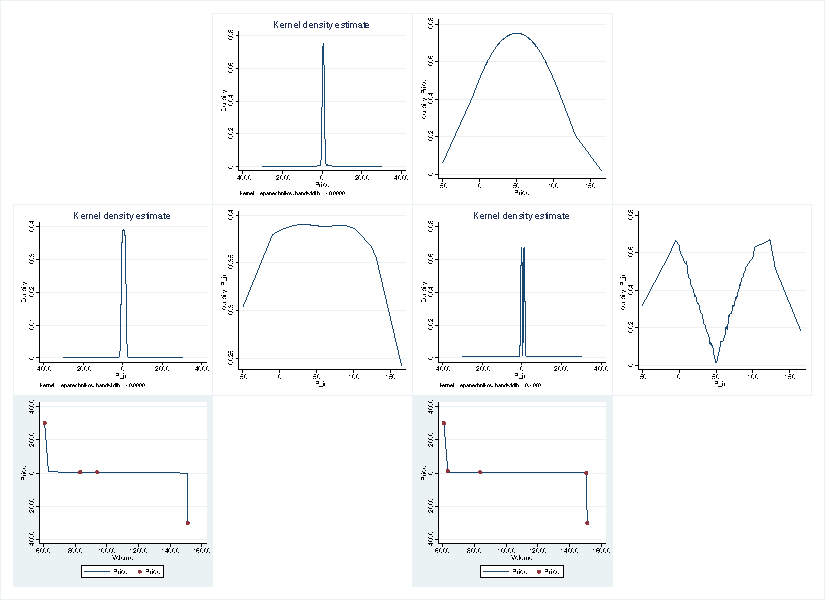
\includegraphics[trim=0.2cm 0.25cm 0.2cm 0.2cm, clip=true, height=90mm]{figch2/comparison1.pdf} 
\caption{Comparison of bandwidths: Large bandwidth in first stage}
\label{bandwidthcomp1}
\end{center}
\emph{Note: Large bandwidth in first stage (top row), large bandwidth in second stage (second row left), small bandwidth in second stage (second row right), Resulting selection of points for large bandwidth in stage one and two (bottow row left, A) and selection of points for large bandwidth in stage one and small bandwidth in stage two (bottom row right, B).}
\end{figure}


\begin{figure}[!ht]
\begin{center}
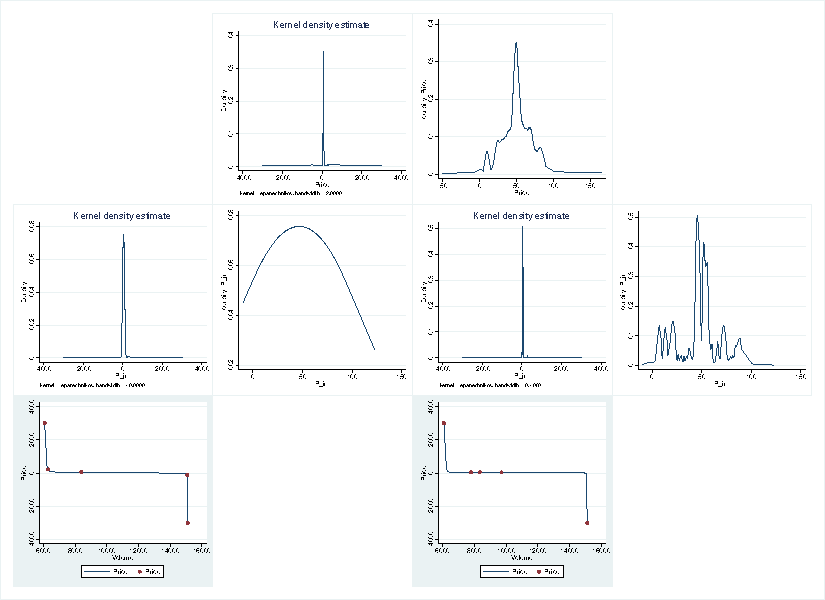
\includegraphics[height=90mm]{figch2/comparison2.pdf} 
\caption{Comparison of bandwidths: Small bandwidth in first stage}
\label{bandwidthcomp2}
\end{center}
\emph{Note: Small bandwidth in first stage (top row), large bandwidth in second stage (second row left), small bandwidth in second stage (second row right), Resulting selection of points for large bandwidth in stage one and small bandwidth in stage two (bottom row left, C) and selection of points for small bandwidth in stage one and two (bottow row right, D).}
\end{figure}


In these graphs, the top row shows the first stage KDE, over the whole function on the left and zoomed on the right. The large bandwidth in figure \ref{bandwidthcomp1} shows the impact of smoothing on the estimates of the first derivative as compared to figure \ref{bandwidthcomp2}.
The second row in both graphs shows the second stage KDE in two versions: Using a wide kernel bandwidth on the left and a tight bandwidth on the right. Again, we disclose the result as seen over the whole function (left) and zoomed on the central price range (right).\\

The third row details the original demand function with the final point selection given the bandwidth selection as given by the two rows above. 
Regardless of the first stage bandwidth, we see that a large bandwidth in the second stage KDE easily distorts the point selection. Selected points of type $k=2,4$ are either two centred or too wide as a result of the second derivatives being smoothed excessively and not precisely representing the local specificities of the curve. \\

The right hand side of both figures show that a tighter bandwidth on the KDE can easily mistake large slope changes due to steps in the bid functions as the appropriate points of maximum curvature of the full bid function and thereby make an error. Therefore, we apply a sensitive second stage KDE on rather smooth estimates of the first derivatives, which yields an adequate point selection in our setting (figure \ref{bandwidthcomp1}B). \\

The bandwidth selection received much attention in this work in order to obtain a reasonable selection of points based on local information of the curves, while achieving a satisfying robustness to noise in the bid function. We are aware that this subjective setting of the bandwidth is not without consequence for our work. However for computational reasons\footnote{The point selection algorithm ran for more than two weeks in the current setting.}, we do not run a full robustness test on this choice ex-post.

\subsection{Outlier detection and removal}
\label{outlier}
In some rare cases, our point selection mechanism does not work. This is the case when curves have very small number of points at a kink and it is thus very difficult to detect their curvature. \\

As a result, the selected points are then quasi in-differentiable from the next selected point type, i.e. a point of type $k=2$ is almost identical to the selected point $k=3$. The code is unable to select the right points due to a data lack on the original curve (second derivative on a constant slope up to POI is zero).\\

We screen for adjacent points that display quasi no variation in volumes. Figure \ref{diff37rangehist} shows a histogram of volumes differences over 2 selected points (from $k=2$ to $k=4$) and reveals a positive mass point at zero, indicating outliers that do not display any volume variation between points of the same bid function. We use the histogram to identify and drop those outliers from our dataset. 

\begin{figure}[!ht]
\begin{center}
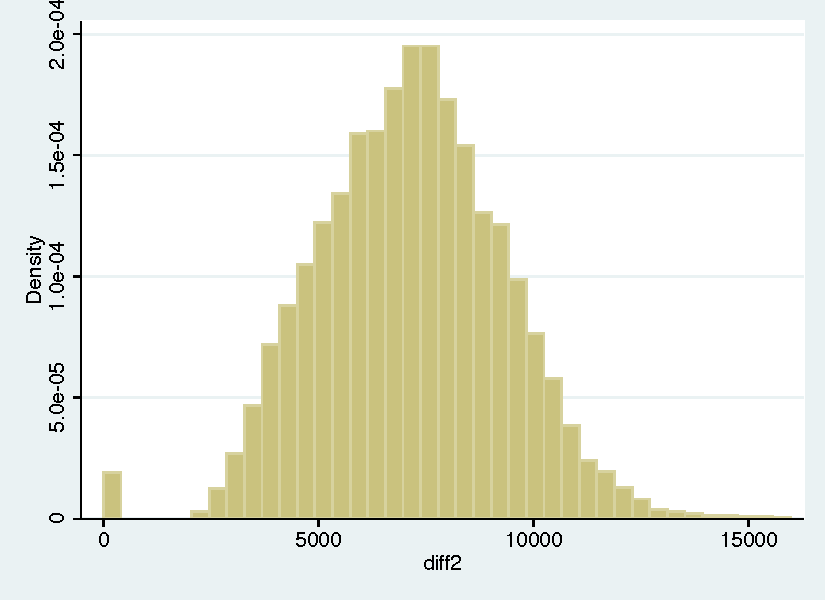
\includegraphics[height=50mm]{figch2/diff37rangehist.pdf} 
\caption{Histogram of volume variation between points}
\label{diff37rangehist}
\end{center}
\emph{Note: The histogram shows the volume difference between points $k=2$ and $k=4$ of the same bid functions. }
\end{figure}

\end{subappendices}












